\documentclass[11pt]{article}
\usepackage[margin=0.9in]{geometry}
\usepackage{amsmath,amssymb,graphicx,booktabs,hyperref,xcolor,float,array,enumitem}
\usepackage[T1]{fontenc}
\usepackage{lmodern}
\usepackage{listings}
\lstset{basicstyle=\ttfamily\scriptsize,breaklines=true,columns=fullflexible,frame=single,language=Python,showstringspaces=false}
\hypersetup{colorlinks=true,linkcolor=blue!60!black,urlcolor=blue!60!black,citecolor=blue!60!black}
\graphicspath{{../v4/}{../v3/}{../v5/}}
\newcommand{\hmpc}{\,h\,\mathrm{Mpc}^{-1}}
\newcommand{\kmax}{k_{\max}}
\newcommand{\kuv}{k_{\rm UV}}
\newcommand{\dchi}{\Delta\chi^2}
\newcommand{\fob}{\mathrm{FoB}}
\newcommand{\rec}[1]{\par\smallskip\noindent\fcolorbox{black!40}{black!4}{\parbox{0.96\linewidth}{\small #1}}\par\smallskip}
\title{Defining intrinsic-alignment scale cuts for NLA and TATT\\[3pt]
\large Strategies, the cuts each one gives, and how to justify the choice\\
(Roman cosmic shear and 3x2pt, FLAMINGO-injected IA)}
\author{Yijie Zhu, with Claude}
\date{10 November 2026}

\begin{document}
\maketitle

\section*{Summary}

This note collects every scale-cut test run over the last week (simulation
fits, the Roman injection tests, mask families, the stitched truth, GGL and
3x2pt) and asks a single question: \emph{what is the right definition of a
scale cut for an IA model, and which cut does each definition give for NLA
and TATT?} Several new calculations were needed to answer it (Sections 2 to 5):
the calibration and noise scatter of the simulation cuts, their dependence on
the simulation volume, a parameter-stability criterion with the correct
variance, the IA accuracy Roman actually requires as a function of $k$, the
precision of every mask, separate cuts for $\xi_+$ and $\xi_-$, and a
theory-error covariance as an alternative to cutting. The main conclusions:

\begin{enumerate}[leftmargin=*,itemsep=2pt]
\item \textbf{Two different questions are being asked, and only one of them
  defines a cut.} ``Where does the model describe the simulation?''
  (simulation-level validity) is a property of the model \emph{and of the
  simulation's volume}: NLA fails at $\kmax \simeq 0.1$ and TATT at
  $0.22$ to $0.39\hmpc$ in FLAMINGO, but the same test with errors scaled to
  Roman's sensitivity gives 0.22 to 0.29 (NLA) and 0.39 to 0.52 (TATT)
  (Sec.~\ref{sec:volume}).
  ``Where is the survey insensitive to the failure?'' (survey-level
  accuracy) is the question a cut must answer. Simulation-level validity is
  evidence for the second question, not a cut by itself.
\item \textbf{At the survey level, with the white term left in the truth,
  NLA and TATT need nearly the same cut}: with the Gaussian covariance both
  reach FoB $= 0.3$ at $K_0 \simeq 0.3$ ($\kuv = K_0/D(z)$); with the
  production covariance \texttt{example1\_cov} at $K_0 \simeq 0.33$ to 0.35
  (Sec.~\ref{sec:ex1}). This is a finding about the white term, not a
  requirement: \textbf{model-specific cuts appear as soon as the white term
  is modelled} (NLA $K_0 \le 0.35$, TATT to 0.5 with \texttt{example1\_cov}),
  for a constant cut (NLA 0.35, TATT 0.4), and for separate $\xi_+$ cuts. The
  redshift shape matters for precision: at equal bias the $1/D$ family is 15
  to 25\% more precise than a constant or $D^{-2/3}$ cut
  (Sec.~\ref{sec:tradeoff}).
\item \textbf{The absolute $S_8$ bias is nearly independent of the cut}
  ($|\delta S_8| \simeq 1.1$ to $2.6\times10^{-3}$ for every mask from 94 to
  385 points, while $\sigma(S_8)$ changes by a factor 6.6). The figure of bias
  rises with $K_0$ because the error bar shrinks, not because more biased
  scales enter. The bias comes from the white (one-halo) II term, which
  enters $\xi_-$ at all angles and which no $k$ cut removes. Cutting hides it
  behind a larger error bar; only modelling removes it (Sec.~\ref{sec:floor}).
\item \textbf{The failure is invisible in the data.} At $K_0 = 0.3$ the
  best-fit $\dchi$ is $\simeq 1$ for 281 points (the $\chi^2$ scatter is 24),
  and the $S_8$ shift between nested cuts is at most $0.3$ of its noise.
  Neither a goodness-of-fit test nor an internal-consistency test on Roman
  data can detect the IA mismodelling, so the cut must be fixed beforehand
  from simulations (Sec.~\ref{sec:detect}).
\item \textbf{Recommendation} (Sec.~\ref{sec:rec}, production covariance).
  Defining criterion: the MAP shift in Roman with every parameter free below
  $0.3\sigma_{\rm 2D}$, $1/D$ masks, model-specific $K_0$. Lens probes
  $K_0^{\rm ggl} = K_0^{\rm gc} = 0.2$, sources behind lenses. For the paper's
  NLA-versus-TATT argument the cleanest set is \emph{one free white-II
  amplitude for both models}: NLA $K_0 = 0.35$ (FoB 0.22, 317 points,
  $\sigma(S_8) = 0.0066$), TATT $K_0 = 0.5$ (FoB 0.24, 385 points,
  $\sigma(S_8) = 0.0055$, 17\% smaller). Without the white term the planned
  $K_0 = 0.35$ is marginal (NLA 0.32, TATT 0.29), and $K_0 = 0.3$ passes for
  both (0.24 / 0.28).
\end{enumerate}

\begin{table}[H]\centering\footnotesize\setlength{\tabcolsep}{3.5pt}
\caption{The strategies at a glance (cosmic shear, production truth, Gaussian
covariance, case A unless stated). ``Cut'': $\kmax(z)$ or $\kuv(z)$ in
$h$/Mpc over $0.2 \le z \le 2$. Roman columns: FoB (in $\sigma$) and
$\sigma(S_8)$ of the mask implied by the cut; ``n/a'' where the cut does not
define a usable Roman mask.}\label{tab:glance}
\resizebox{\textwidth}{!}{%
\begin{tabular}{p{4.6cm}p{2.7cm}p{2.7cm}p{2.5cm}p{5.2cm}}
\toprule
strategy & NLA cut & TATT cut & Roman FoB NLA / TATT, $\sigma(S_8)$ & verdict \\
\midrule
A1 GoF, $p<0.05$ (or $\chi^2/\nu>2$) & 0.09 to 0.12 & 0.22 to 0.39 & NLA-shaped mask: 0.01 (9 pts); TATT-shaped: 0.23 / 0.22 (145 pts, 0.0084) & model validity in this box; volume dependent; too strict for Roman \\
A2 parameter stability (nested) & 0.16 to 0.39 & 0.16 to 0.39 & n/a & blind to failures in the sub-dominant probe (II); calibration in Sec.~\ref{sec:stab} \\
A3 accuracy 10\% (GI and II) & 0.09 to 0.12 & 0.22 to 0.39 & as A1 & tolerance arbitrary unless derived from the survey (B2) \\
A4 $k_{\rm NL}(z)$ & 0.31 to 2.3 & same & n/a & the IA cuts do not follow $k_{\rm NL}$; rejected \\
\midrule
B1 $\dchi_{\rm Roman} < 1$, no refit & flat $\simeq 0.27$ & flat $\simeq 0.29$ & 0.23 / 0.22 (flat 0.29) & sensible, model specific; ignores parameter projection \\
B2 required accuracy $\varepsilon(k)$ & see Fig.~\ref{fig:tol} & see Fig.~\ref{fig:tol} & n/a & turns A3 into a survey statement; useful for the paper's narrative \\
B3 Roman refit $\chi^2 < 1$ & $K_0 \simeq 0.28$ & $K_0 \simeq 0.31$ & $\simeq$0.27 / 0.35 & close to C, but undetectable $\neq$ unbiased \\
\midrule
C FoB $<0.3$, all parameters free & $K_0 \simeq 0.30$ ($1/D$); flat 0.3 & $K_0 \simeq 0.28$; flat 0.3 & 0.30, $\sigma(S_8)=0.0049$ & what the chains measure; the baseline definition \\
C$'$ FoB $+ \sigma_{\rm noise} < 0.3$ & $K_0 \simeq 0.25$ & $K_0 \simeq 0.2$ to 0.25 & 0.23 / 0.26, 0.0060 & conservative version, accounts for FLAMINGO noise \\
C$''$ separate $\xi_+$, $\xi_-$ cuts & $K_0^\pm = 0.3, 0.25$ & $K_0^\pm = 0.4$, $\le0.15$ & 0.23 / 0.16, 0.0052 / 0.0054 & the bias lives in $\xi_-$; TATT earns $\xi_+$ scales \\
\midrule
D1 white-II nuisance $+$ C & $K_0 \le 0.35$ & $K_0 \le 0.5$ & 0.17 / 0.14 at 0.35 & removes the bias floor; TATT gains scales \\
D2 theory-error covariance & see Sec.~\ref{sec:theory} & see Sec.~\ref{sec:theory} & & reduces but does not remove the bias with the measured envelope \\
\bottomrule
\end{tabular}}
\end{table}

\section{What a scale cut has to do}\label{sec:req}

A scale cut is a statement of the form ``with this model, these data points
can be used without biasing the parameters we report''. That sentence
contains four requirements, and every strategy below can be judged by them.

\begin{description}[leftmargin=1.2em,itemsep=2pt]
\item[R1 Accuracy.] The bias on the reported parameters, here $(\Omega_m,
  S_8)$, from the IA model's failure on the kept scales is below a stated
  threshold. This is the only requirement that is about the result; the
  others are about whether R1 can be trusted.
\item[R2 Robustness.] R1 holds for the plausible range of IA truths, not
  just for one simulation: different galaxy selections, the white term in or
  out, the stitched versus measured spectra, simulation noise.
\item[R3 Efficiency.] Among the cuts that satisfy R1 and R2, the one that
  keeps the most information (smallest $\sigma(S_8)$ or largest FoM).
\item[R4 Transparency.] The cut is defined by a rule that can be written in
  one sentence and re-applied to another survey, model or probe without
  re-running the full analysis; it does not reward a model for absorbing
  the residual in a nuisance direction.
\end{description}

Two further properties are desirable for this paper in particular: the cut
should allow a fair comparison of NLA and TATT (R5: a better model should be
able to earn smaller scales), and the cut should be the same object for
cosmic shear, GGL and clustering (R6).

\paragraph{The two questions.} The tests of the last week fall into two groups.
\emph{Simulation-level} tests ask whether a model describes the FLAMINGO
spectra (goodness of fit, parameter stability, fractional accuracy).
\emph{Survey-level} tests ask whether the failure matters for Roman (the
$\dchi$ translation, the figure of bias). Only the second group speaks to
R1. The first group answers ``where is the model physically valid?'', which
is useful context (and is what an IA paper should report about the models),
but it depends on the simulation's statistical power rather than the
survey's, as Sec.~\ref{sec:volume} makes quantitative.

\paragraph{Definitions used throughout.}
Simulation fits: per snapshot $s$, $\chi^2(\kmax) = \sum_{X}\sum_{0.05\le
k_i\le\kmax}[(y_{s,X} - M_{s,X})/\sigma_{s,X}]^2$ over $X \in \{hE, EE,
BB\}$, $N_s$ fixed to the B plateau, $\nu = 3N_k - n_{\rm par}$
($n_{\rm par} = 1$ for NLA, 3 for TATT). Masks: IR/UV masks with $\alpha =
0.05$ on GG plus an NLA baseline, $\kuv(z) = K_0\,D(z)^{-p}$ with $p = 1$
(production), $2/3$, or 0 (constant), or the simulation cuts interpolated in
$z$ and multiplied by $f$. Roman: $\xi_\pm$, 1080 points, Gaussian
covariance; truth $=$ GG $+$ FLAMINGO IA through \texttt{sim\_IA}; the model
is fitted with $\Omega_m$, $A_s$ (case A; case B adds $n_s$, $H_0$,
$\Omega_b$ with Gaussian priors of the chain-prior width) and all IA
parameters free, and the figure of bias is
\begin{equation}
\fob = \sqrt{\delta\theta^{\rm T}\,\Sigma_\theta^{-1}\,\delta\theta},
\qquad \theta = (\Omega_m, S_8),
\label{eq:fob}
\end{equation}
with $\delta\theta$ the best-fit (MAP) shift and $\Sigma_\theta$ the Fisher
covariance with the IA parameters marginalised over a Gaussian of the flat
prior width. The matched-model control (TATT on a TATT truth) is zero to three
decimals at every mask, so every nonzero FoB here is model mismatch.

\section{Strategy family A: validity of the model in the simulation}\label{sec:A}

\subsection{A1 Goodness of fit}\label{sec:gof}
\paragraph{Definition.} $p(\kmax) = P[\chi^2_\nu > \chi^2_{\min}(\kmax)]$;
the cut is the last $\kmax$ before two consecutive $p < 0.05$. Equivalently,
$\chi^2_{\min}/\nu > \chi^2_{0.95}(\nu)/\nu$ (1.4 to 2.6 depending on
$\nu$); a fixed $\chi^2/\nu > 2$ gives the same cuts within one grid step
(companion note of 9 November).

\paragraph{Result.} NLA 0.09 to 0.12, TATT 0.22 to 0.39 (Fig.~\ref{fig:cuts}),
nearly flat in $z$; core combined 0.09 (NLA) and 0.22 (TATT).

\paragraph{Calibration.} If the model were exactly right, how often would
the rule cut anyway? Realisations of a truth that \emph{is} the model (NLA
fitted to the smoothed truth at $k\le0.16$; TATT at $k\le0.29$) plus
FLAMINGO noise give a false-cut rate (two consecutive failures before
$k = 2.27$) of 9.8\% per snapshot for NLA and 10.8\% for TATT
(Table~\ref{tab:calib}), and in 61 to 65\% of the realisations at least one
of the nine core snapshots cuts spuriously (median spurious cut 0.16). The
two-consecutive requirement is weaker than it looks because the tests are
nested: $\chi^2(k_j)$ contains $\chi^2(k_{j-1})$, so a failure is usually
followed by another. A toy with $\chi^2$ increments of 3 dof per node gives
8 to 9\% per snapshot, the same. Two consequences: per-snapshot cuts must
be smoothed in $z$ (a power law in $D(z)$, or the core-combined test, whose
false-cut rate is 8 to 11\%) rather than read one by one; and a significance
threshold of $p = 0.05$ per test corresponds to roughly $p = 0.1$ per
snapshot.

\paragraph{Noise scatter.} Over 300 realisations of FLAMINGO noise around
the smoothed truth the per-snapshot cut has a typical 16 to 84\% range of
$<0.09$ to 0.12 (NLA) and 0.16 to 0.29 (TATT) (Fig.~\ref{fig:noise},
Table~\ref{tab:calib}), one to two grid steps (factors of 1.35 in $k$). The
realisations are centred one step below the measured cuts for TATT: the
spline used as the truth carries some structure of its own at low $k$, so
the medians are pessimistic and only the widths should be used. The cuts in
Fig.~\ref{fig:cuts} carry that resolution.

\paragraph{The volume dependence.}\label{sec:volume}
The goodness of fit is a significance: it asks whether the residual is
detectable \emph{with FLAMINGO's error bars}. With the true residual fixed,
a box of $f$ times the volume has errors $\sigma/\sqrt f$ and an expected
\begin{equation}
\langle\chi^2_{\min}\rangle(\kmax; f) \simeq \nu + f\,\hat\lambda(\kmax),\qquad
\hat\lambda = \chi^2_{\rm meas} - \nu ,
\label{eq:vol}
\end{equation}
with $\hat\lambda$ the non-centrality estimated from the measured spectra
($\hat\lambda$ is unbiased if the noise is Gaussian with the quoted errors).
Applying the $p$ rule to Eq.~(\ref{eq:vol}) gives the cut as a function of
$f$ (Fig.~\ref{fig:volume}): core combined, NLA moves from 0.09 ($f = 1$)
to 0.12 ($f = 1/4$), 0.16 ($f = 1/16$) and 0.22 ($f = 1/32$); TATT from 0.22
($f = 1$) to 0.29 ($f = 1/8$) and 0.39 ($f = 1/32$). A larger simulation
makes both models fail earlier, without limit: any parametric model is
rejected at any $k$ by a large enough box. The cut a GoF test returns is
thus a statement about FLAMINGO L1000, not about Roman.

Roman's sensitivity to the same residuals is $\dchi_{\rm Roman}/\dchi_{\rm
FL} \simeq 0.02$ to $0.04$ for fits with $\kmax \le 0.22$ (the translation
matrix of the main summary). Reading Fig.~\ref{fig:volume} at
$f = 0.02$ to $0.04$ gives NLA 0.22 to 0.29 and TATT 0.39 to 0.52: a
significance cut ``with Roman's eyes'' lands in the range of the
survey-level cut of Sec.~\ref{sec:C} ($\kuv = 0.3/D(z)$, i.e.\ 0.33 at
$z = 0.2$ to 0.49 at $z = 1$; a constant 0.3), with NLA on the tight side
and TATT on the loose side. The two models are still distinguished, but by
much less than the factor 2.5 of the raw FLAMINGO test. This is the cleanest way to
connect the simulation fits to the survey, and the strongest argument
against using the raw GoF cut as the Roman cut.

\begin{figure}[H]\centering
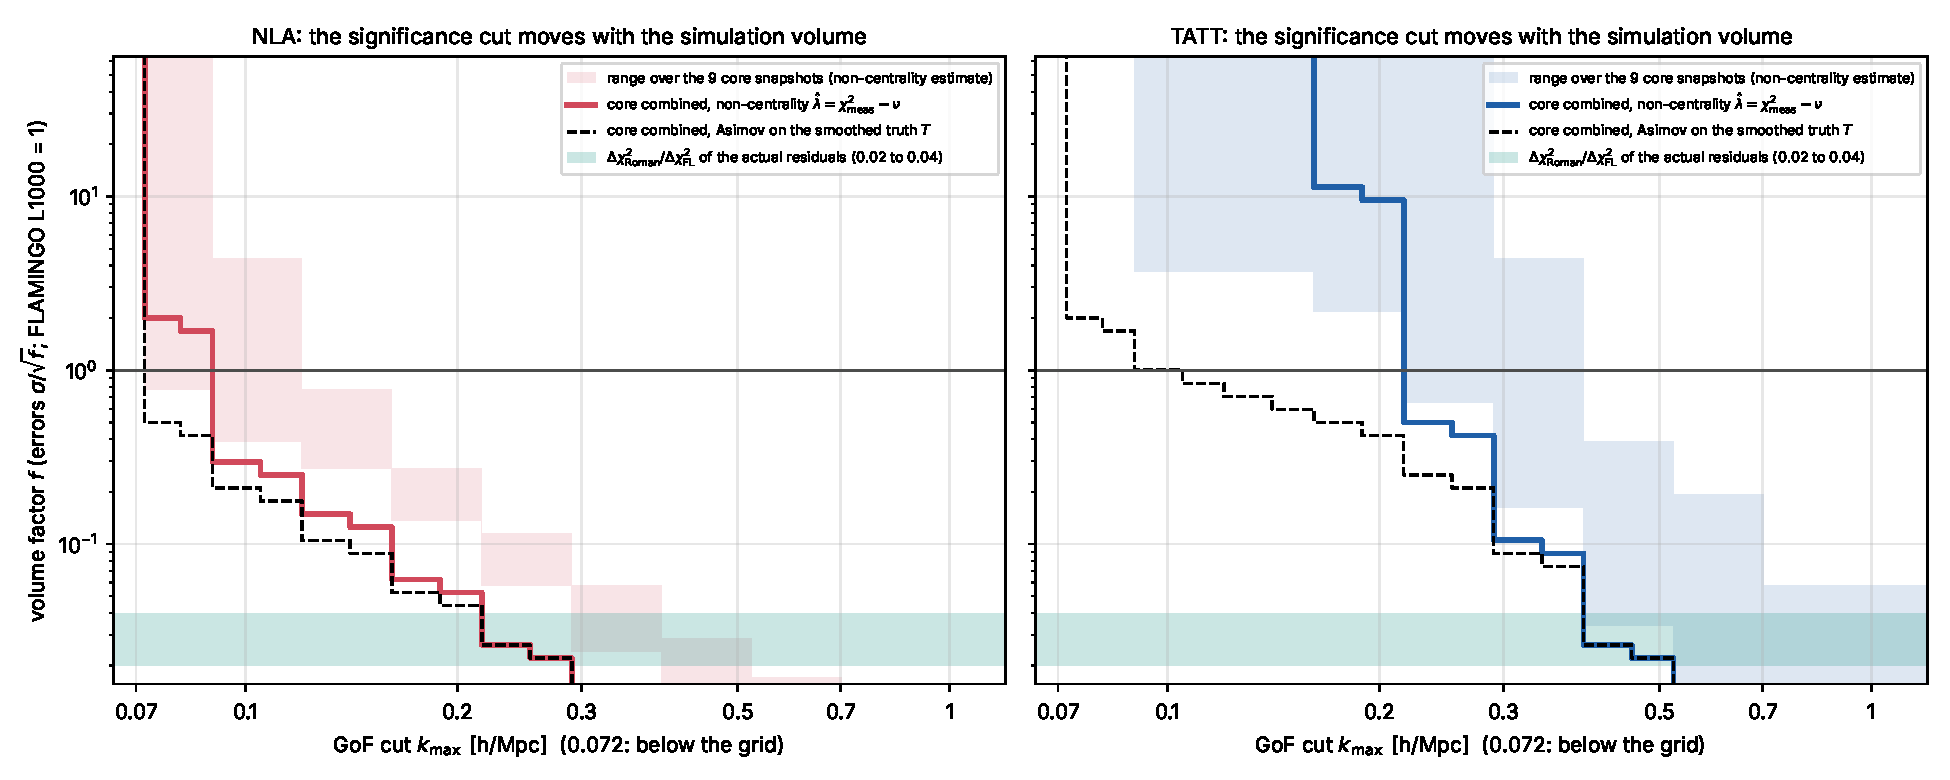
\includegraphics[width=\textwidth]{fig_strat_volume}
\caption{The goodness-of-fit cut against the simulation volume factor $f$
($k$ horizontal). Thick: core combined from the non-centrality estimate
Eq.~(\ref{eq:vol}); band: range over the nine core snapshots; dashed: the
same with the smoothed truth $T$ as an Asimov data set (the spline carries
extra structure at low $k$, so this version is stricter). Green band: the
ratio of Roman to FLAMINGO $\dchi$ for the actual NLA/TATT residuals.
$\hat\lambda$ is set to zero where $\chi^2_{\rm meas} < \nu$, which is why
the curves stop moving at large $f$; the true cut would keep moving in.}
\label{fig:volume}
\end{figure}

\rec{\textbf{A1 verdict.} Report it as the range of validity of each model
in FLAMINGO (it is what distinguishes TATT from NLA physically: a factor 2.5
in $\kmax$). Do not use it as the Roman cut: it is set by the box's volume,
it gives NLA 9 usable $\xi_\pm$ points, and the same test at Roman's
sensitivity agrees with the survey-level cut.}

\subsection{A2 Parameter stability}\label{sec:stab}
\paragraph{Definition.} The idea is to cut where the fitted amplitude stops
being stable as smaller scales are added. Three versions:
\begin{itemize}[itemsep=1pt]
\item \emph{naive, fixed reference}: fail at $\kmax$ if
  $|a_1(\kmax) - a_1(0.09)| > \sigma_{a_1}(0.09)$;
\item \emph{naive, sequential}: fail if $|a_1(k_j) - a_1(k_{j-1})| > \sigma_{a_1}(k_{j-1})$;
\item \emph{nested}: the fits at $k_{j-1}$ and $k_j$ use nested data, so
  under a correct model the difference of the two estimates has covariance
  \begin{equation}
  \mathrm{Cov}(\hat\theta_{j-1} - \hat\theta_j) = V_{j-1} - V_j
  \label{eq:nested}
  \end{equation}
  (the larger data set's estimate is uncorrelated with the difference; this
  is the Hausman test). Fail if $\Delta^{\rm T}(V_{j-1}-V_j)^{+}\Delta >
  \chi^2_{0.95}(n_{\rm par})$, all fitted parameters.
\end{itemize}
All with the two-consecutive-failure rule. The naive versions use the wrong
variance: $\sigma_{a_1}(k_{\rm ref})$ is the error of one estimate, not of the
difference, and for a correct model $|a_1(\kmax) - a_1(k_{\rm ref})|$ exceeds
$\sigma_{a_1}(k_{\rm ref})$ with probability up to 32\% at every $\kmax$.

\paragraph{Results.} Fig.~\ref{fig:cuts}, Table~\ref{tab:calib}. Nested
test: NLA 0.16 at $z \le 0.5$, 0.29 to 0.39 at $z$ = 0.6 to 1, 0.22 and 0.16
at $z$ = 1.5 and 2; TATT 0.16 to 0.39 with no trend. The naive reference
test gives NLA 0.12 to 0.52 and erratic TATT values (0.09 to 0.39). False-cut
rates on a model truth: nested 2.4\% (NLA, well calibrated) and 12\% (TATT,
where bounded parameters, $b_{\rm TA} = 0$ in particular, break the Gaussian
approximation behind Eq.~\ref{eq:nested}); naive sequential 7.5\%; naive
reference 24 to 37\% per snapshot and 89 to 98\% for at least one core
snapshot. The naive reference version cuts somewhere almost always, even when
the model is exact.

\paragraph{Why NLA looks stable.} The NLA amplitude is set almost entirely
by GI, whose fractional errors are 2.5 to 4 times smaller than those of II
(5 to 15 times the $\chi^2$ weight). NLA's GI
residual is small until $k \simeq 0.3$ (the dip of $P_{\delta E}/P_{\rm NL}$
starts there), so $a_1$ stays put while the II prediction is already 20 to
30\% low (companion note, Fig.~3 to 6). Parameter stability tests the
probe that dominates the parameter, not the model: it is blind to the
failure in the sub-dominant probe, which in this case is exactly the failure
that biases Roman (the II white term). TATT's three parameters drift more
visibly, and its stability cut is close to its GoF cut.

\rec{\textbf{A2 verdict.} If a stability criterion is used, use the nested
variance Eq.~(\ref{eq:nested}); the ``$1\sigma$ of the lower-$k$ value''
version has no fixed false-alarm rate. Even then it is a weaker test than
the GoF for NLA (it ignores II) and adds nothing for TATT. Not recommended as
the defining criterion; worth one sentence in the paper as a cross-check.}

\subsection{A3 Fractional accuracy}
\paragraph{Definition and result.} The anchored model ($k \le 0.16$) within
5\% or 10\% of the smoothed truth for GI and II up to $\kmax$. 10\%: NLA 0.09
to 0.12, TATT 0.22 to 0.39; the 5\% II criterion is never met by either
model because of the white excess. The tolerance is not tied to anything:
Sec.~\ref{sec:tolerance} replaces it with the tolerance Roman actually
requires.

\subsection{A4 A physical scale}
$k_{\rm NL}(z)$ ($\Delta^2_{\rm lin} = 1$) runs from 0.31 at $z = 0.2$ to 2.3
at $z = 2$ ($k_{\rm NL} \propto D^{-2.6}$), while the measured IA cuts are
flat (NLA, $p = 0.05\pm0.21$) or grow as $D^{-2/3}$ (TATT, $p = 0.66 \pm
0.21$); $\kmax/k_{\rm NL}$ falls from 0.4 to 0.05 (NLA) and 0.7 to 0.17
(TATT). Whatever limits the models is set by halo-scale (one-halo)
physics, not by where matter goes non-linear. A cut at a fixed fraction of
$k_{\rm NL}$ would over-reach at high $z$ by a factor 3 or more.

\begin{figure}[H]\centering
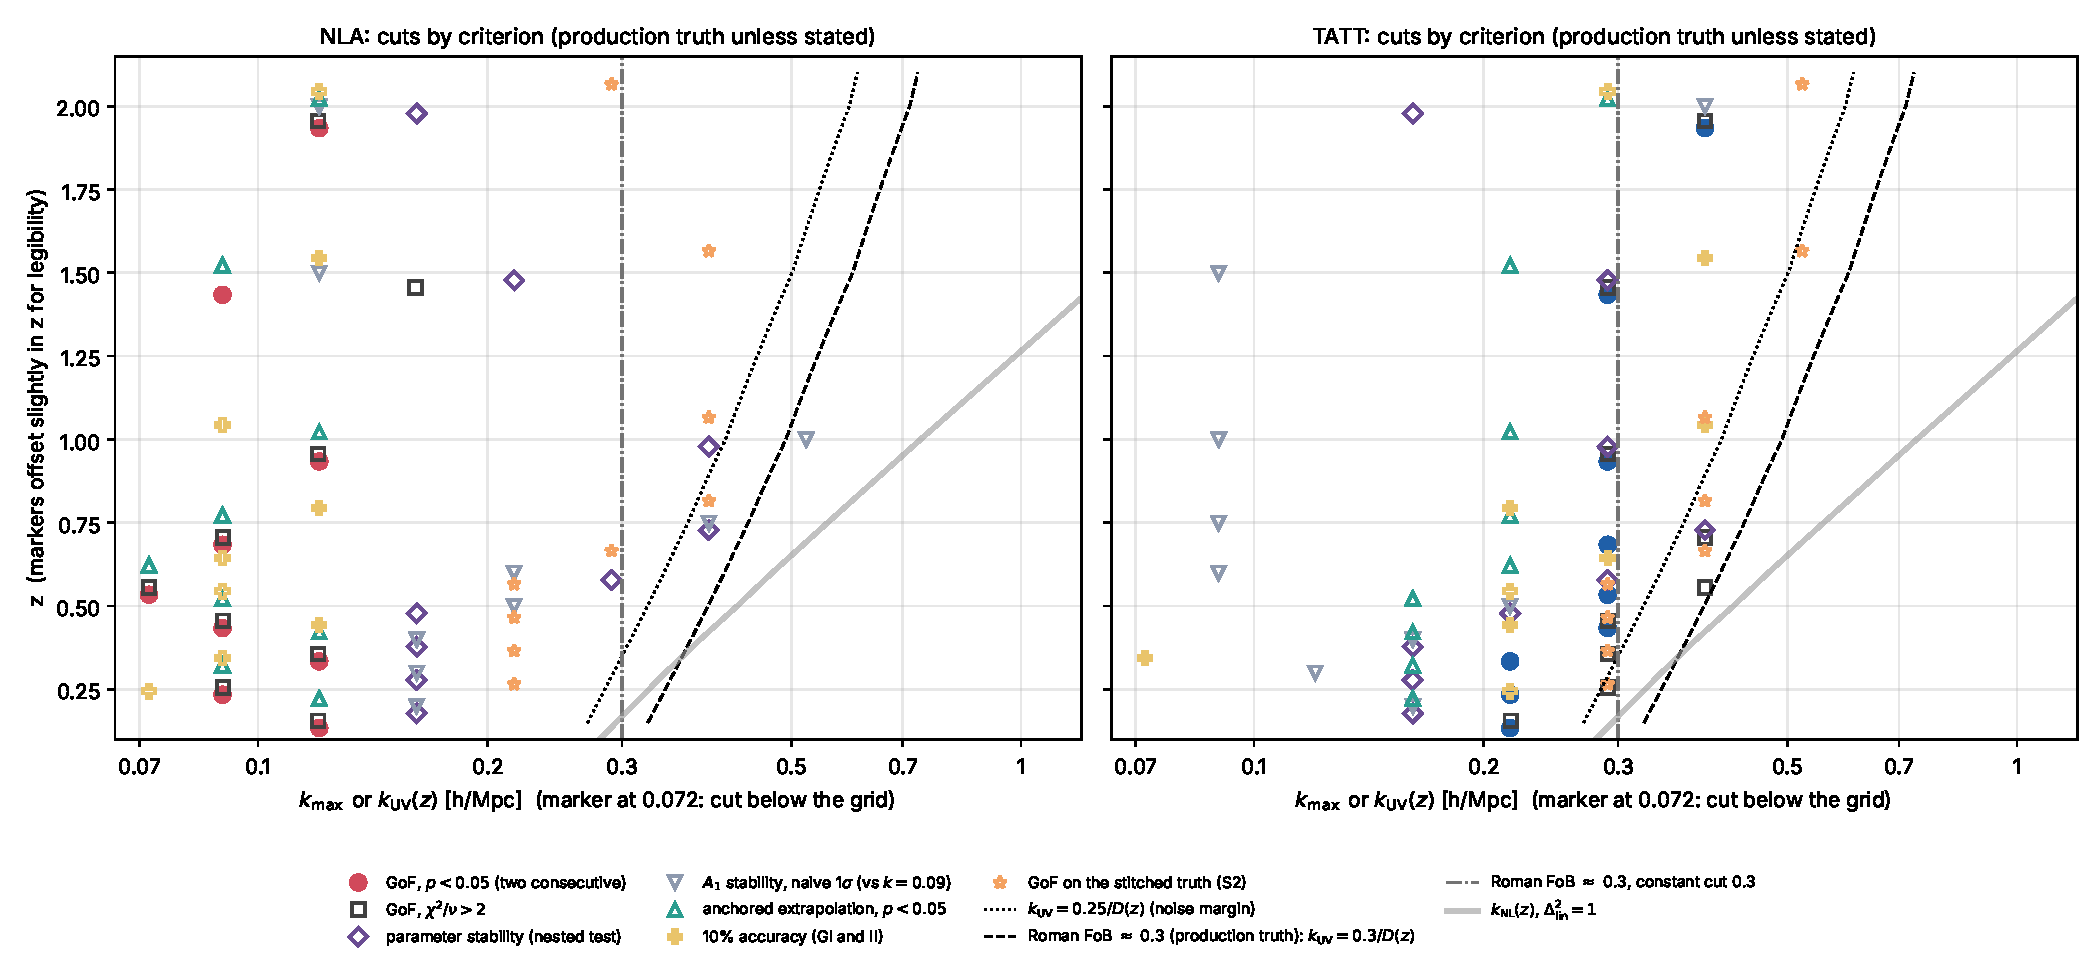
\includegraphics[width=\textwidth]{fig_strat_cuts}
\caption{Cuts by criterion ($k$ horizontal, $z$ vertical; markers offset in
$z$ by up to $\pm0.07$ for legibility). Filled circles: GoF; open symbols:
$\chi^2/\nu > 2$, parameter stability (nested and naive), anchored
extrapolation, 10\% accuracy, GoF on the stitched truth. Lines: the Roman
FoB $=0.3$ mask in the $K_0/D$ family ($K_0 = 0.3$, dashed) with the
noise-margin version ($K_0 = 0.25$, dotted), the constant cut 0.3, and
$k_{\rm NL}(z)$.}
\label{fig:cuts}
\end{figure}

\begin{figure}[H]\centering
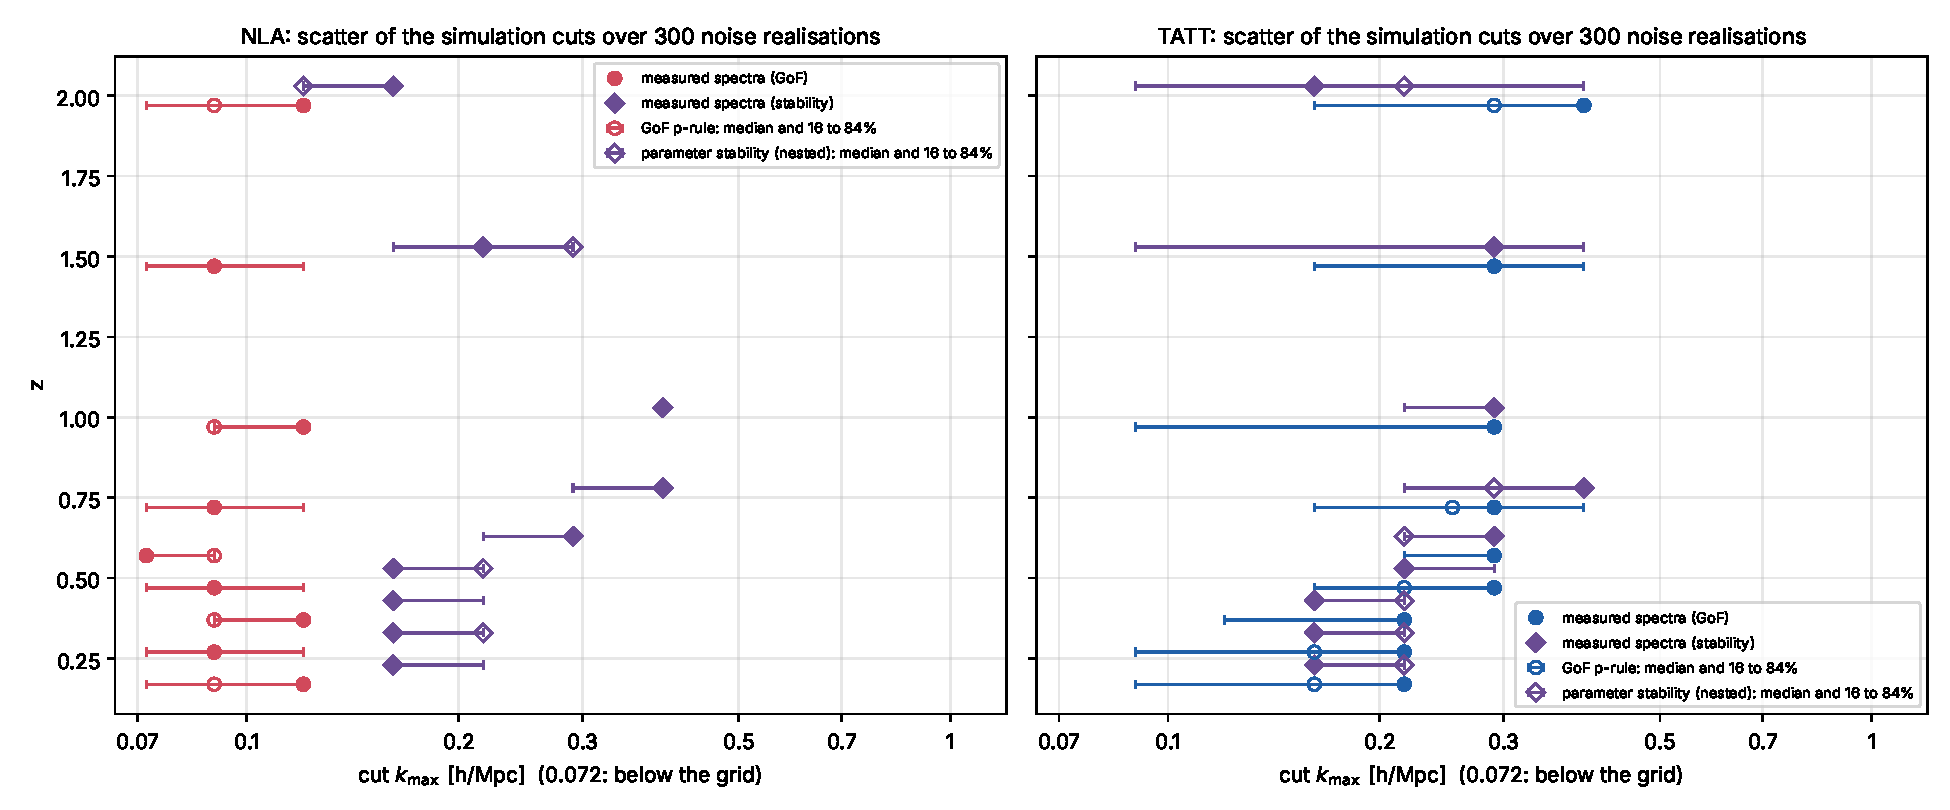
\includegraphics[width=\textwidth]{fig_strat_noise}
\caption{Scatter of the simulation cuts over noise realisations around the
smoothed truth (median and 16 to 84\%), GoF and nested stability, with the
cuts of the measured spectra.}
\label{fig:noise}
\end{figure}

\begin{table}[H]\centering\small
\caption{Calibration and noise scatter of the simulation rules (300
realisations each). ``False-cut rate'': fraction of snapshot fits that cut
before $k = 2.27$ when the truth is the model itself; ``any core'': at least
one of the nine core snapshots cuts; ``16 to 84\%'': range of the cut over
realisations of FLAMINGO noise around the smoothed truth (median over the
core snapshots of the 16th and 84th percentiles).}
\label{tab:calib}
\resizebox{\textwidth}{!}{\begin{tabular}{l rrr rrr}\toprule
 & \multicolumn{3}{c}{NLA} & \multicolumn{3}{c}{TATT}\\ \cmidrule(lr){2-4}\cmidrule(lr){5-7}
rule & false-cut rate & any core & 16 to 84\% & false-cut rate & any core & 16 to 84\%\\ \midrule
GoF $p$-rule & 9.8\% & 61\% & $<$0.09 to 0.12 & 10.8\% & 65\% & 0.16 to 0.29\\
$a_1$ stability, naive (vs 0.09) & 37.4\% & 98\% & 0.12 to 0.22 & 23.9\% & 89\% & 0.09 to 0.39\\
$a_1$ stability, naive sequential & 7.6\% & 53\% & 0.16 to 0.22 & 7.5\% & 49\% & 0.12 to 0.29\\
stability, nested test & 2.4\% & 20\% & 0.16 to 0.22 & 12.0\% & 76\% & 0.16 to 0.29\\
\midrule
GoF, core combined & 8.0\% &  & $<$0.09 to $<$0.09 & 11.3\% &  & $<$0.09 to 0.16\\
\bottomrule\end{tabular}}
\end{table}

\section{Strategy family B: the simulation misfit seen by Roman}\label{sec:B}

\subsection{B1 Survey-weighted misfit without refitting}
\paragraph{Definition.} Take the IA amplitudes fitted in FLAMINGO at
$\kmax(z)$, compute the Roman $\xi_\pm$ of model and truth with the same
amplitudes, and require $\dchi_{\rm Roman} = \Delta\xi^{\rm T}C^{-1}\Delta\xi
< 1$ on the mask built from $\kmax(z)$ (DES Y3 cosmic shear used
$\dchi = 0.5$ for baryons \cite{secco22}).

\paragraph{Result} (main summary, Table 6). Masks shaped like the TATT
simulation cut, scaled by $f$: $\dchi_{\rm Roman}$ = 0.22 / 0.14 (NLA /
TATT) at $f = 0.7$ (flat 0.20), 1.51 / 0.98 at $f = 1$ (flat 0.29), 11.5 /
7.0 at $f = 1.4$ (flat 0.40). Interpolating in $\ln\dchi$, $\dchi = 1$ is reached at
$\kuv(z{=}1) = 0.27$ (NLA) and 0.29 (TATT); $\dchi = 0.5$ at 0.24 and
0.26.
This criterion is model specific (TATT's residual is smaller), cheap, and
needs only the cell Jacobian. Its weakness is the one the Roman test
removes: it does not let the cosmology and IA parameters respond, so it
neither credits the model for absorbing part of the residual nor charges it
for projecting the rest onto $S_8$.

\subsection{B2 The accuracy Roman requires}\label{sec:tolerance}
\paragraph{Definition.} Perturb the FLAMINGO IA spectra by a coherent
fractional error $\varepsilon$ at every $k' \ge k$ (a step), in GI, II or
both, propagate with the cell Jacobian $\mathsf{J}=\partial\xi_\pm/\partial
P_X(k_i,z_s)$, and find the $\varepsilon$ that gives $\dchi_{\rm Roman} = 1$
on a given mask, or FoB $= 0.3$ through the linear estimator with the IA
parameters refitted:
\begin{equation}
\delta\xi = \varepsilon\,\mathsf{J}\,(T\,\mathbb{1}_{k'\ge k}),\qquad
\dchi = \delta\xi^{\rm T}C^{-1}\delta\xi,\qquad
\delta\theta = \mathsf{G}\,(\mathsf{F}^{-1}\mathsf{J}_\theta^{\rm T}C^{-1})\,\delta\xi .
\label{eq:tol}
\end{equation}
($\mathsf{J}_\theta$: Jacobian in cosmology and IA parameters, $\mathsf{F}$
the Fisher matrix with priors, $\mathsf{G}$ the projection on
$(\Omega_m, S_8)$.)

\paragraph{Result} (Fig.~\ref{fig:tol}). On the $K_0 = 0.3$ mask Roman
requires a coherent GI error above $k$ to stay below 7\% for $k \ge 0.12$,
10\% for $k \ge 0.16$, 17\% for $k \ge 0.29$ and 38\% for $k \ge 0.52$;
for II the numbers are 14, 18, 22 and 48\%. The requirement relaxes by a factor
$\simeq 1.5$ from $K_0 = 0.4$ to $0.2$ only. The FoB-based tolerance is
noisier (it depends on how the perturbation projects on the IA and cosmology
directions, so it jumps between neighbouring $k$) but of the same order.
Compared with what the models achieve when anchored at $k\le0.16$: NLA's GI
is within the requirement everywhere, NLA's II is at the requirement from
$k \simeq 0.12$ and above it from $k \simeq 0.29$; TATT is within it on
average for both GI and II at all $k$ shown, although its worst snapshot
exceeds the GI requirement from $k \simeq 0.4$. This is the survey-aware replacement for A3, and it
is a good figure for the paper: it shows in one panel why the II white term,
not the GI shape, is what matters for Roman, and how much better TATT would
have to be to buy more scales.

\begin{figure}[H]\centering
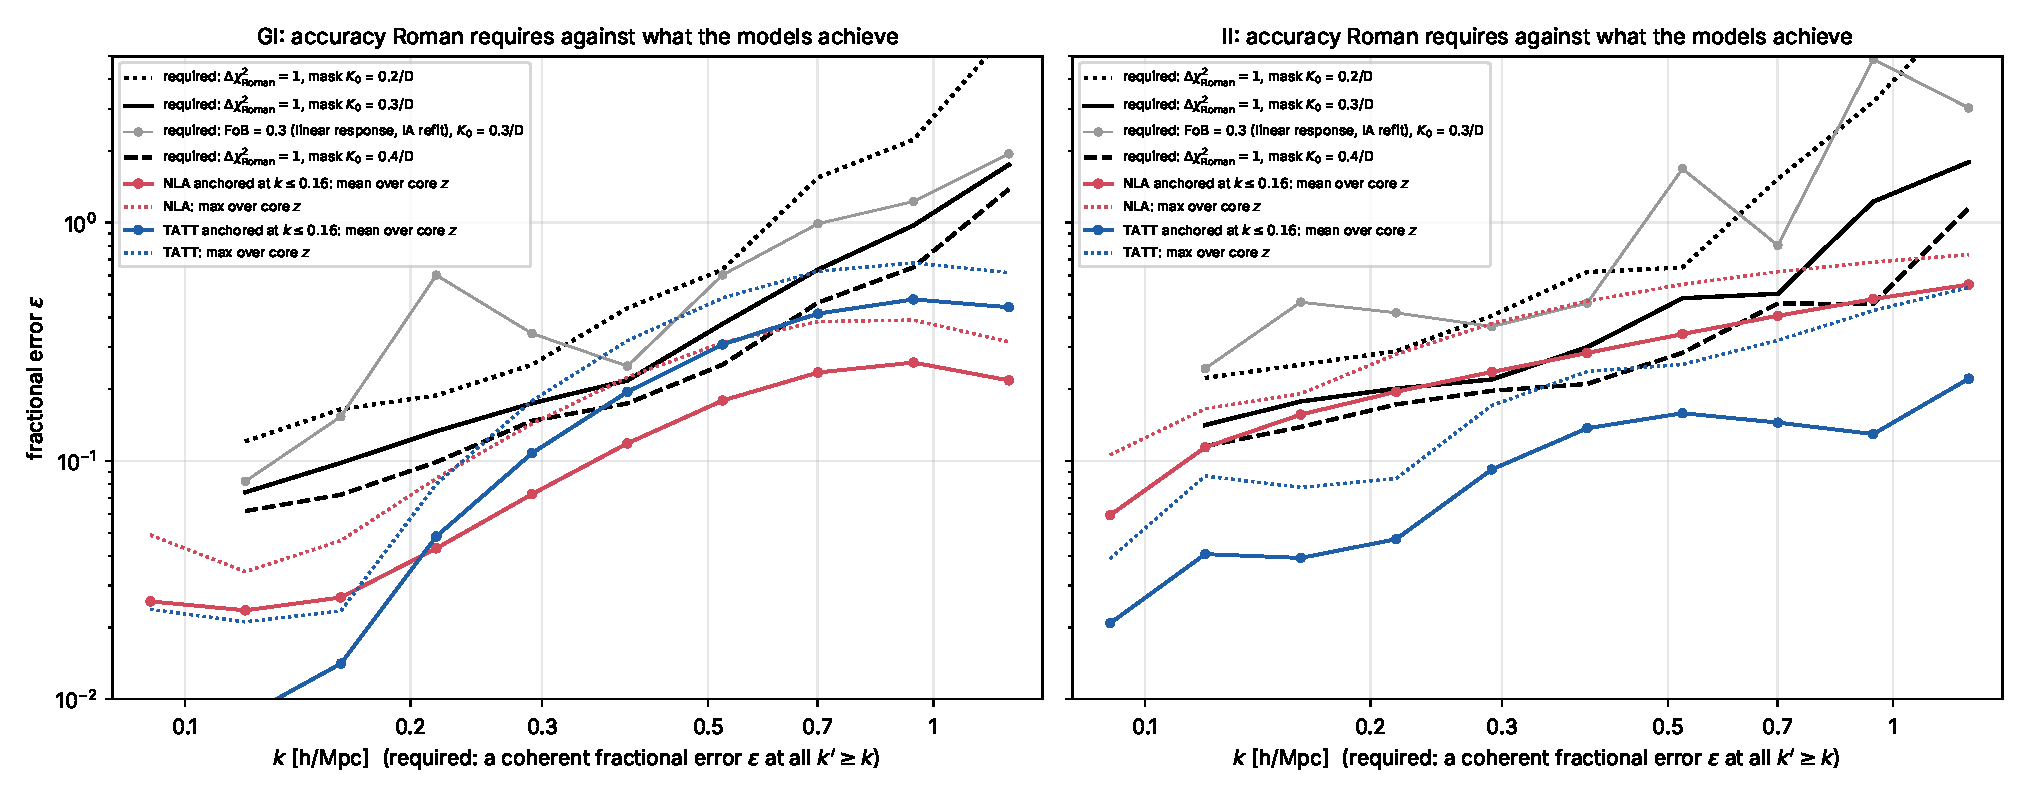
\includegraphics[width=\textwidth]{fig_strat_tolerance}
\caption{Required accuracy: the coherent fractional error at all $k' \ge
k$ that gives $\dchi_{\rm Roman} = 1$ (black: masks $K_0 = 0.2$, 0.3, 0.4 in
the $1/D$ family) or FoB $=0.3$ with the IA refitted (grey, $K_0 = 0.3$),
against the measured error of the NLA and TATT fits anchored at $k \le 0.16$
(mean and maximum over the core snapshots). Left GI, right II.}
\label{fig:tol}
\end{figure}

\subsection{B3 Survey-level goodness of fit, and what it cannot do}\label{sec:detect}
The Roman best-fit $\chi^2$ (data noiseless, so this is the $\dchi$ the
mismodelling adds) reaches 1 at $K_0 \simeq 0.28$ (NLA) and $0.31$ (TATT),
close to the FoB crossing. Requiring $\dchi_{\rm Roman,\,refit} < 1$ is
therefore a fair proxy for C on this truth. But it should not be confused with
detectability. With $N$ points the data $\chi^2$ scatters by $\sqrt{2N}$: 24 at
$N = 281$. A misfit of $\dchi \simeq 1$ to 2.5 (the range of every mask up to
$K_0 = 0.5$) is $0.04$ to $0.1\sigma$ of that scatter and will never be seen in
the data. The same holds for internal consistency between cuts: the $S_8$
shift between consecutive masks of the $1/D$ family is $-0.07$ to $+0.32$
times the expected noise of the difference, $\sqrt{\sigma^2_{\rm small} -
\sigma^2_{\rm large}}$ (Table~\ref{tab:cons}). Both tests a real analysis
would run are blind to this systematic.

\rec{\textbf{B verdict.} B1 and B2 are the right way to report the
simulation results in survey terms, and B2 makes a good figure. Neither is
the final criterion, because the reported parameters are fitted. The
failure is undetectable in Roman data, which is why the cut has to be set
from simulations before unblinding and cannot be validated afterwards.}

\begin{table}[H]\centering\small
\caption{Internal consistency between consecutive masks ($1/D$ family, case
A): change of the FLAMINGO-induced $S_8$ shift between the two masks, the
expected noise of that change for nested data, and their ratio.}
\label{tab:cons}
\begin{tabular}{llrrrrr}\toprule
model & masks & $\delta S_8$ small & $\delta S_8$ large & change & noise of change & ratio\\ \midrule
NLA & 0.2 $\to$ 0.25 & +0.0016 & +0.0013 & -0.0003 & 0.0041 & -0.07\\
NLA & 0.25 $\to$ 0.3 & +0.0013 & +0.0015 & +0.0001 & 0.0036 & +0.04\\
NLA & 0.3 $\to$ 0.35 & +0.0015 & +0.0018 & +0.0003 & 0.0016 & +0.17\\
NLA & 0.35 $\to$ 0.4 & +0.0018 & +0.0024 & +0.0007 & 0.0021 & +0.32\\
NLA & 0.4 $\to$ 0.5 & +0.0024 & +0.0021 & -0.0003 & 0.0020 & -0.18\\
TATT & 0.2 $\to$ 0.25 & +0.0014 & +0.0015 & +0.0001 & 0.0041 & +0.02\\
TATT & 0.25 $\to$ 0.3 & +0.0015 & +0.0015 & +0.0001 & 0.0035 & +0.02\\
TATT & 0.3 $\to$ 0.35 & +0.0015 & +0.0019 & +0.0004 & 0.0017 & +0.21\\
TATT & 0.35 $\to$ 0.4 & +0.0019 & +0.0024 & +0.0005 & 0.0019 & +0.27\\
TATT & 0.4 $\to$ 0.5 & +0.0024 & +0.0022 & -0.0002 & 0.0022 & -0.07\\
\bottomrule\end{tabular}
\end{table}

\section{Strategy family C: the parameter shift in Roman}\label{sec:C}

\subsection{Definition and result}
\paragraph{Definition.} The cut is the largest mask whose FoB
(Eq.~\ref{eq:fob}) stays below a threshold $\tau$ when the model is fitted
to the FLAMINGO-injected data vector with every parameter free and the chain
priors, after checking that the matched-model control is zero. This is
precisely what the chains will measure (MAP), so it is the definition that
answers R1 directly, and it is the convention of DES Y3 (FoB $< 0.3\sigma_{\rm
2D}$ in $(\Omega_m, S_8)$ for 3x2pt \cite{krause21,secco22}).

\paragraph{Result} (main summary, Sections 7 and 11). FoB $= 0.3$ at
$K_0 \simeq 0.3$ for both models in both cases in the $1/D$ family (281
points), at $K_0 \simeq 0.27$ for $D^{-2/3}$, and at a constant
$\kuv \simeq 0.3$ to $0.35$. Cases A and B agree to $\pm0.07$. The FLAMINGO
noise on the FoB is $\pm0.06$ to $0.09$.

\subsection{The threshold}\label{sec:threshold}
Three considerations fix $\tau$.
\begin{itemize}[itemsep=2pt]
\item \emph{Coverage.} A shift of $b\sigma$ in one parameter lowers the
  coverage of the 68\% interval to $\Phi(1-b) - \Phi(-1-b)$: 0.683, 0.680,
  0.661, 0.625 for $b$ = 0, 0.1, 0.3, 0.5. $\tau = 0.3$ costs 2 points of
  coverage, $0.5$ costs 6.
\item \emph{Budget.} The 0.3 of DES Y3 was for the total of the modelling
  systematics tested (baryons for shear; baryons plus non-linear bias for
  3x2pt), not for each one. If IA, baryons and non-linear bias each take an
  equal share in quadrature, IA gets $0.3/\sqrt3 = 0.17$.
\item \emph{Simulation noise.} The FoB is measured on one box with
  $\pm0.07$ uncertainty; requiring FoB $+\,\sigma_{\rm noise} < 0.3$ (C$'$)
  moves the cut one step in, to $K_0 = 0.25$ for NLA and between 0.2 and
  0.25 for TATT.
\end{itemize}
With $\tau = 0.17$ no useful $1/D$ mask passes ($K_0 = 0.15$: 0.17 / 0.14,
$\sigma(S_8) = 0.011$, 2.3 times the error of $K_0 = 0.3$). This is the
practical consequence of the next subsection.

\subsection{The bias floor}\label{sec:floor}\label{sec:tradeoff}
Fig.~\ref{fig:trade} plots the FoB of every mask of the three families
against its precision $\sigma(S_8)$ (Fisher, case A, validated against the
fits to 1 to 5\%). The masks fall close to curves of constant
\emph{absolute} bias, $\fob \simeq |\delta S_8|/\sigma(S_8)$ with
$|\delta S_8| \simeq 1.1$ to $2.6 \times 10^{-3}$, over a range in which
$\sigma(S_8)$ changes from 0.023 to 0.0035. In words: the $S_8$ bias the
FLAMINGO IA induces is about $2\times10^{-3}$ whatever the cut; cutting does
not reduce it, it only enlarges the error bar until the bias is no longer
significant. The white II term explains this (main summary, Sec.~5): a
white $P_{EE}$ gives a constant $C_\ell$ and $\xi_- = 2C/(\pi\theta^2)$ at
all $\theta$, a large-angle signal that a $k$ cut cannot remove. The linear
response to the white term alone gives $|\delta S_8| \simeq 0.4$ to
$1.5\times10^{-3}$ on the same masks, about half of the total.

Consequences: (i) the FoB threshold is a statement about $\sigma(S_8)$, not
about $k$: the cut passes $\tau = 0.3$ once $\sigma(S_8) \gtrsim
2\times10^{-3}/0.3 \simeq 0.005$ to 0.007, whatever the shape of the mask;
(ii) with the white term in the truth, a stricter budget can only be met by
throwing away precision; (iii) the efficient frontier is the family that
reaches a given $\sigma(S_8)$ with the least bias: at FoB $= 0.3$,
$\sigma(S_8) = 0.0049$ (NLA) and 0.0054 (TATT) for $1/D$, 0.0061 and
0.0064 for $D^{-2/3}$, 0.0057 and 0.0064 for a constant cut. The $1/D$
family is the most efficient by 15 to 25\%, because it
cuts hardest at low redshift, where the $\xi_-$ white tail of the low-$z$ bins
lives.

\begin{figure}[H]\centering
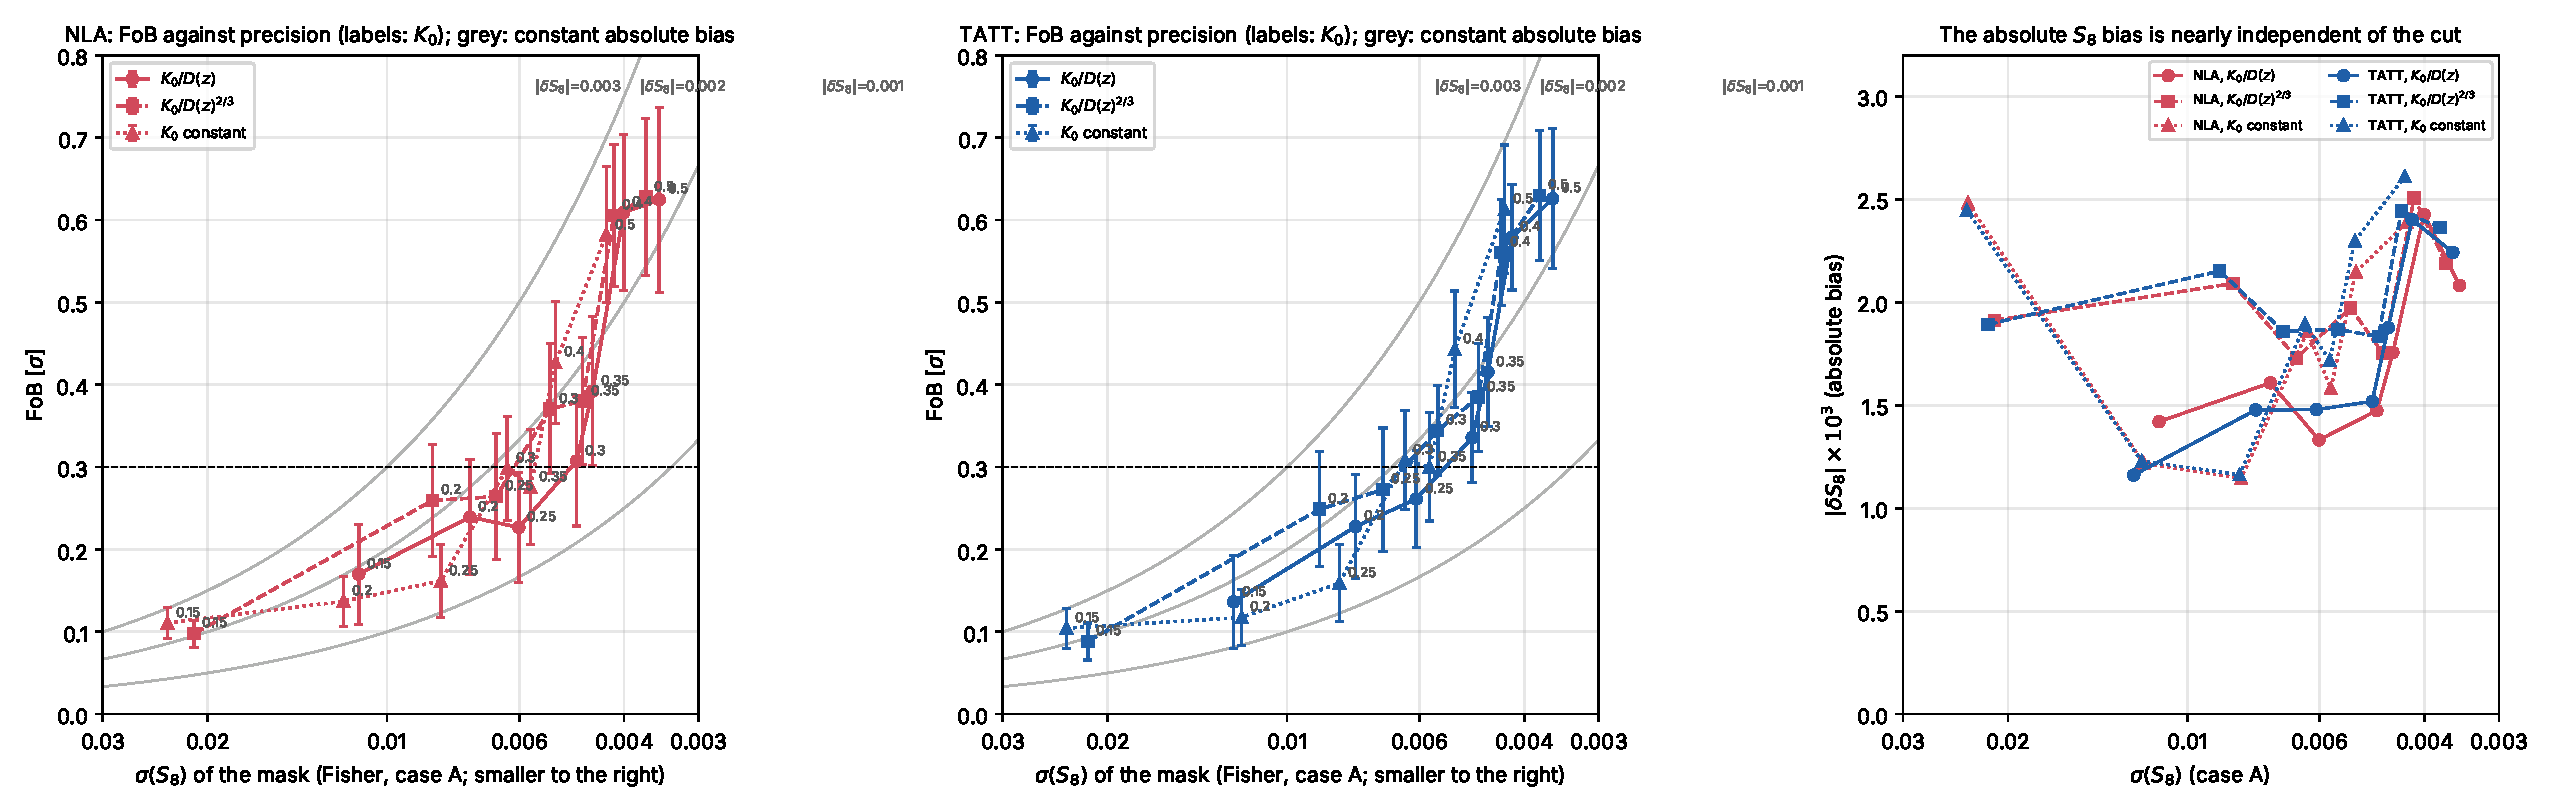
\includegraphics[width=\textwidth]{fig_strat_tradeoff}
\caption{Left, middle: FoB against $\sigma(S_8)$ of the mask (Fisher, case
A; precision increases to the right) for the three families (labels:
$K_0$), with FLAMINGO-noise error bars; grey: constant absolute bias
$|\delta S_8|$ = 0.001, 0.002, 0.003. Right: $|\delta S_8|$ itself.}
\label{fig:trade}
\end{figure}

\subsection{Separate cuts for $\xi_+$ and $\xi_-$}\label{sec:split}
The floor comes from $\xi_-$ (a white $C_\ell$ is invisible in $\xi_+$ at
$\theta > 0$), so the two correlation functions need not share $K_0$.
Fig.~\ref{fig:split} scans masks that take the $\xi_+$ rows from $K_0^+$ and
the $\xi_-$ rows from $K_0^-$ (both $1/D$ family; $K_0^- = 0$ drops $\xi_-$),
with the linear-response FoB (IA refitted, case A), which reproduces the full
fits on the diagonal to $\pm0.04$. Selected masks were refitted in full
(Table~\ref{tab:split}).
\begin{itemize}[itemsep=2pt]
\item \textbf{$\xi_-$ sets the bias.} At fixed $K_0^+$ the FoB rises with
  $K_0^-$ in every row; at fixed $K_0^-$ it barely moves with $K_0^+$ up to
  0.35.
\item \textbf{$\xi_+$ separates the models.} With $\xi_-$ restricted, NLA's
  FoB jumps from 0.22 to 0.39 between $K_0^+ = 0.35$ and 0.4, while TATT
  stays at 0.19 to $K_0^+ = 0.4$ and 0.28 at 0.5 (no $\xi_-$). This is the
  GI dip of $P_{\delta E}/P_{\rm NL}$ at $k \simeq 0.3$ to 1 that TATT follows
  and NLA does not (companion note, Fig.~1 to 3), seen by Roman.
\item \textbf{Precision.} At equal bias the separate cuts are 13 to 20\%
more precise than the common $1/D$ cut. NLA: $(K_0^+, K_0^-) = (0.3, 0.25)$
gives FoB 0.23 (0.25 in case B) with $\sigma(S_8) = 0.0052$, against 0.23
and 0.0060 for the common $K_0 = 0.25$; $(0.35, 0.25)$ gives 0.27 / 0.29
with 0.0050. TATT: $(0.4, {\rm no}\ \xi_-)$ gives 0.16 / 0.13 with
$\sigma(S_8) = 0.0054$, against 0.26 / 0.30 and 0.0061 for the common
$K_0 = 0.25$; $(0.5, {\rm no}\ \xi_-)$ gives 0.30 / 0.17. Keeping
$\xi_-$ to $K_0^- = 0.25$ with $K_0^+ = 0.4$ is fine in case A (0.28) but
not in case B (0.41), so for TATT the robust choice drops the small-scale
$\xi_-$ ($K_0^- \le 0.15$; linear FoB 0.21 at $K_0^- = 0.15$). NLA fails at
$K_0^+ = 0.4$ whatever $\xi_-$ does (0.39 / 0.37 with no $\xi_-$). For TATT
the Fisher $\sigma(S_8)$ of the scan is evaluated at one IA point and can
differ from the full fit by up to 50\% where the best fit moves far from it
($(0.5, {\rm none})$: 0.0042 against 0.0066); the full fits are the numbers
to quote.
\end{itemize}
Separate cuts therefore satisfy R5 without any extra nuisance parameter: the
better model earns more $\xi_+$ scales. The cost is a second free number per
probe, and a mask choice that is driven by where the white term lives; the
latter should be stated as such.

\begin{figure}[H]\centering
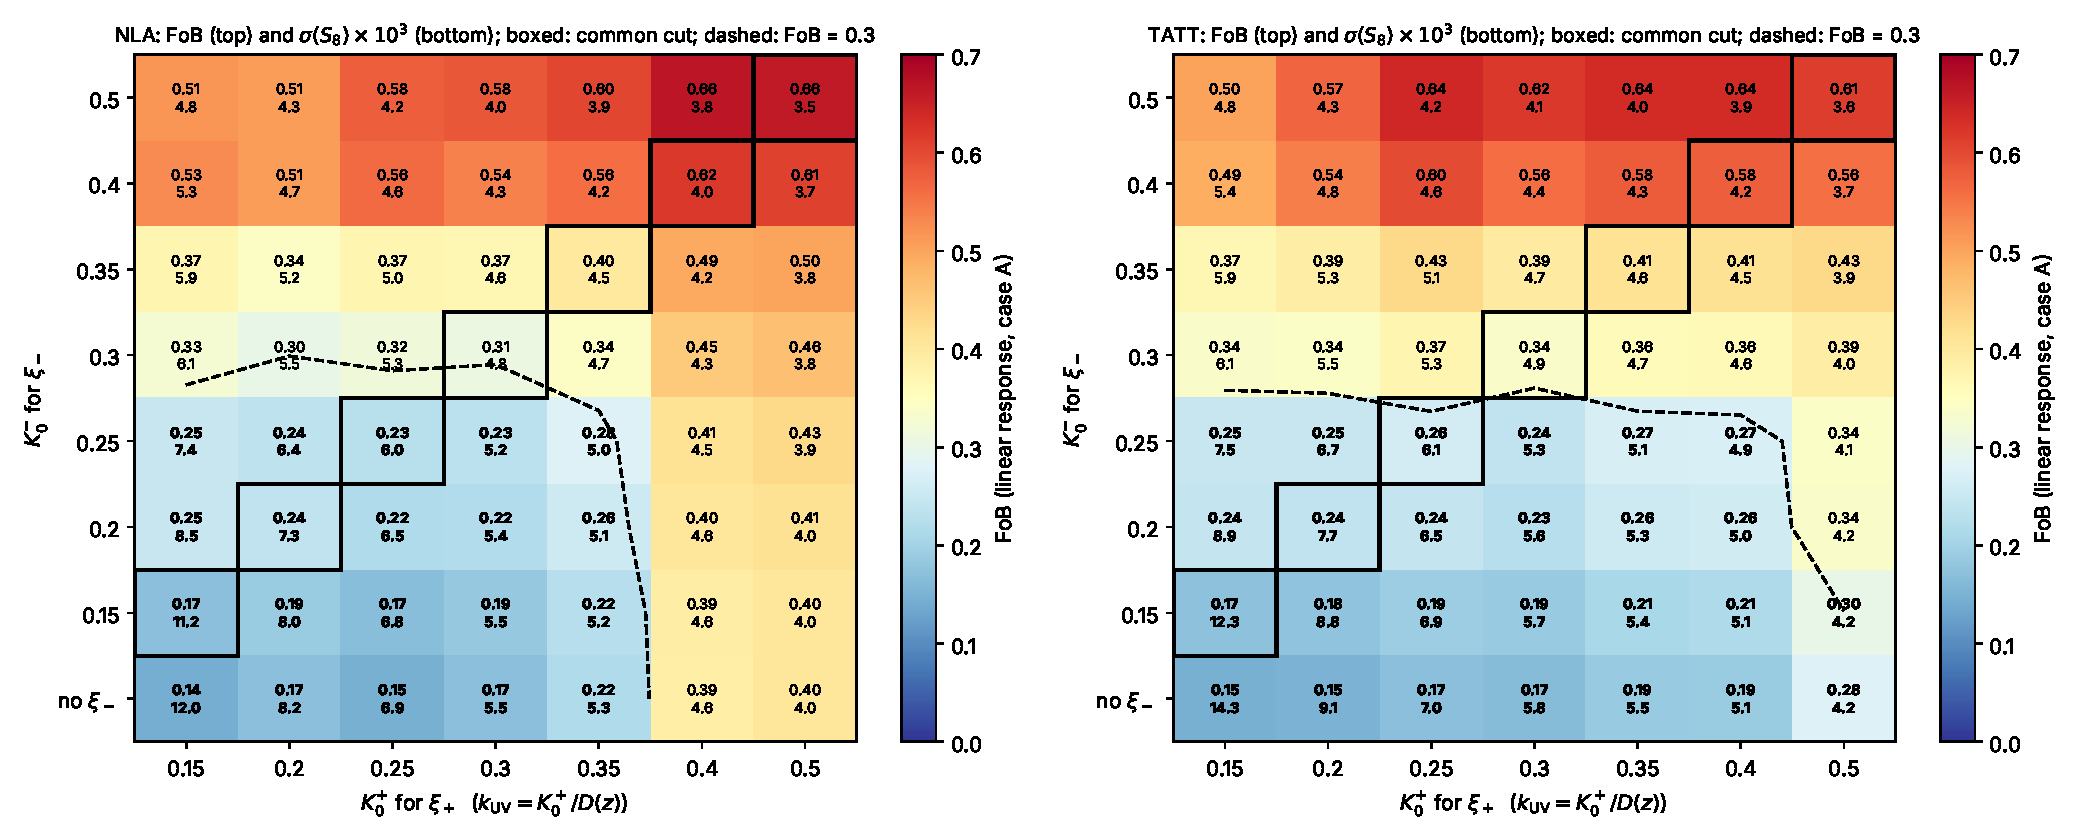
\includegraphics[width=\textwidth]{fig_strat_split}
\caption{Separate cuts for $\xi_+$ ($K_0^+$, horizontal) and $\xi_-$
($K_0^-$, vertical): FoB (colour and upper number, bold if below 0.3) and
$\sigma(S_8)\times10^3$ (lower number), linear response with IA refitted,
case A. Boxed: the common-cut masks of Sec.~\ref{sec:C}.}
\label{fig:split}
\end{figure}

\begin{table}[H]\centering\small
\caption{Full non-linear fits at separate $\xi_\pm$ masks (all parameters
free; $\pm$: FLAMINGO noise).}
\label{tab:split}
\begin{tabular}{lcc r ccc cc}\toprule
model & $K_0^+$ & $K_0^-$ & pts & FoB A & FoB B & $\chi^2$ A & $\sigma(S_8)$ A & linear FoB\\ \midrule
NLA & 0.3 & 0.25 & 265 & 0.23 $\pm$ 0.08 & 0.25 & 0.98 & 0.0052 & 0.23\\
NLA & 0.35 & 0.25 & 290 & 0.27 $\pm$ 0.09 & 0.29 & 1.25 & 0.0050 & 0.28\\
NLA & 0.5 & none & 293 & 0.39 $\pm$ 0.13 & 0.29 & 1.74 & 0.0040 & 0.40\\
TATT & 0.4 & none & 263 & 0.16 $\pm$ 0.05 & 0.13 & 0.77 & 0.0054 & 0.19\\
TATT & 0.4 & 0.25 & 299 & 0.28 $\pm$ 0.05 & 0.41 & 1.10 & 0.0049 & 0.27\\
TATT & 0.5 & none & 293 & 0.30 $\pm$ 0.09 & 0.17 & 1.01 & 0.0066 & 0.28\\
\bottomrule\end{tabular}
\end{table}

\subsection{Projection and the chain}
The MCMC at $K_0 = 0.3$ (main summary, Sec.~7) reproduced the MAP shifts and
showed a $0.24\sigma$ prior-volume shift of the TATT posterior mean even on a
TATT truth. Strategy C must therefore be stated for the MAP, or for the
posterior mean minus the matched-model control. Otherwise TATT, with its
weakly constrained $\eta_2$ and $b_{\rm TA}$, is charged with a projection
effect that is not model failure and would need a tighter cut than NLA for
reasons unrelated to IA physics.

\rec{\textbf{C verdict.} The defining criterion. State it as: ``the
largest $\kuv$ for which the MAP shift of $(\Omega_m, S_8)$ from the
FLAMINGO-injected data vector, with all parameters free, stays below
$0.3\sigma_{\rm 2D}$ (FoB $+$ its simulation-noise uncertainty)''. On the
production truth: $K_0 = 0.25$ in the $1/D$ family for both models, or the
separate $\xi_\pm$ cuts of Sec.~\ref{sec:split}. Be explicit that the bias
does not go to zero at smaller $K_0$.}

\section{Strategy family D: model the residual instead of cutting it}\label{sec:D}

\subsection{D1 One nuisance for the white II term}
Adding a free amplitude $a_w$ for the white II template (the measured
$\xi_\pm$ signature of the excess) removes the floor (main summary,
Sec.~11): $1/D$ family FoB 0.11 / 0.11 at $K_0 = 0.3$, 0.17 / 0.14 at 0.35,
then NLA fails (0.40 at 0.4) while TATT stays at 0.21 to 0.28 up to $K_0 =
0.5$; a constant cut stays at or below 0.12 for both models to $k = 0.5$. Its
cost in precision is small: $\sigma(S_8)$ grows by 1 to 8\% in the $1/D$
family (case A; 2 to 10\% in case B) and by up to 18\% for a constant cut
at 0.5 (Fisher with $a_w$ marginalised, flat prior width $10/\sqrt{12}$).
At $K_0 = 0.35$ with $a_w$, $\sigma(S_8) = 0.0048$ (NLA) and 0.0049 (TATT):
20\% better than the cut-only baseline at $K_0 = 0.25$ (0.0060), with a
smaller bias. The white term is the low-$k$ limit of a one-halo
alignment term: any one-halo contribution tends to a constant as $k \to 0$,
so the template is the leading term of a halo-model IA description rather
than an ad hoc fix. This is also the configuration in which TATT earns
smaller scales than NLA, which is what a model comparison paper should be able
to show (R5).

\subsection{D2 Theory-error covariance}\label{sec:theory}
\paragraph{Definition.} Keep the scales and add the model error to the
covariance \cite{baldauf16,chudaykin21}:
\begin{equation}
C \to C + \mathsf{J}\,\Sigma_{\rm th}\,\mathsf{J}^{\rm T},\qquad
(\Sigma_{\rm th})_{ab} = e_a e_b\,\rho_k(a,b)\,\rho_z(a,b)\,\delta_{X_aX_b},
\label{eq:th}
\end{equation}
with $e_a = E_X(k_a)\,|T_a|$ the envelope of the model's fractional error
(measured: $\max_z |M/T - 1|$ of the anchored fit, made monotonic in $k$),
Gaussian correlations of width 0.5 in $\ln k$ and in $z$, GI and II
uncorrelated.

\paragraph{Result} (Table~\ref{tab:theory}). Each model with its own
envelope (NLA anchored at $k \le 0.16$, TATT at $k \le 0.29$). The FoB in
units of the inflated error drops by 15 to 40\% (0.31 to 0.26 and 0.34 to
0.25 at $K_0 = 0.3$; from 0.58 to 0.62 down to 0.37 to 0.47 at $K_0 = 0.4$
and 0.5),
$\sigma(S_8)$ grows by 10 to 30\%, and the shift in units of the
statistical error stays at 0.27 to 0.28 ($K_0 = 0.3$) and 0.44 to 0.53
($K_0 \ge 0.4$). The theory error down-weights the scales where the
envelope is large, but the bias comes from the white term at low $k$, where
the measured envelope is only a few per cent, so it is not removed. With the
envelope set by one simulation, D2 performs like a slightly softer cut at
$K_0 \simeq 0.3$; it would become useful with an envelope spanning several
IA truths.

\begin{table}[H]\centering\small
\caption{Theory-error covariance (Eq.~\ref{eq:th}), case A: FoB in units of
the inflated $\sigma$, $\sigma(S_8)$, and best-fit $\chi^2$, with and
without $C_{\rm th}$.}
\label{tab:theory}
\begin{tabular}{llrrrrrr}\toprule
 & & \multicolumn{3}{c}{statistical $C$} & \multicolumn{3}{c}{$C + C_{\rm th}$}\\ \cmidrule(lr){3-5}\cmidrule(lr){6-8}
model & mask & FoB & $\sigma(S_8)$ & $\chi^2$ & FoB & $\sigma(S_8)$ & $|\delta S_8|/\sigma_{\rm stat}$\\ \midrule
NLA & $K_0/D$ 0.3 & 0.31 & 0.0048 & 1.18 & 0.26 & 0.0053 & 0.28\\
NLA & $K_0/D$ 0.4 & 0.61 & 0.0040 & 1.90 & 0.46 & 0.0046 & 0.53\\
NLA & $K_0/D$ 0.5 & 0.62 & 0.0035 & 2.53 & 0.43 & 0.0042 & 0.51\\
NLA & constant 0.5 & 0.58 & 0.0043 & 1.82 & 0.47 & 0.0046 & 0.50\\
TATT & $K_0/D$ 0.3 & 0.34 & 0.0049 & 0.96 & 0.25 & 0.0058 & 0.27\\
TATT & $K_0/D$ 0.4 & 0.58 & 0.0042 & 1.55 & 0.41 & 0.0051 & 0.49\\
TATT & $K_0/D$ 0.5 & 0.63 & 0.0036 & 2.06 & 0.38 & 0.0047 & 0.49\\
TATT & constant 0.5 & 0.61 & 0.0043 & 1.45 & 0.37 & 0.0052 & 0.44\\
\bottomrule\end{tabular}
\end{table}

\rec{\textbf{D verdict.} D1 is cheap (one linear parameter), physically
motivated, and the only option that removes the bias floor and lets the
model comparison show up in Roman. D2 with an envelope measured on the same
simulation is a softer version of a cut; it is the natural language for a
future analysis with several simulations defining the envelope, not the
baseline here.}

\section{Model-specific or common cuts?}
The simulation says TATT is valid to 2.5 times larger $k$ than NLA (A1).
Roman, on the production truth, says both need the same cut (C), because
the bias is the white term that neither model has. Three ways to frame this
in the paper, in order of preference:
\begin{enumerate}[itemsep=2pt]
\item \textbf{Common cut, model the white term} (D1): one mask for both
  models at $K_0 = 0.35$, then show that TATT stays unbiased to $K_0 = 0.5$
  while NLA does not. This uses the simulation result and makes the NLA/TATT
  comparison a Roman statement.
\item \textbf{Separate $\xi_\pm$ cuts, no white term} (Sec.~\ref{sec:split}):
  $\xi_-$ cut where the white term allows ($K_0^- \simeq 0.15$ to 0.25),
  $\xi_+$ cut per model (NLA 0.3 to 0.35, TATT 0.4 to 0.5). The model
  difference appears in $\xi_+$, where the GI shape matters, and costs no
  extra parameter.
\item \textbf{Common cut, no white term} (C$'$): $K_0 = 0.25$ for both;
  report that TATT's better fit to FLAMINGO does not translate into
  less bias, and explain why (the floor).
\item \textbf{Model-specific simulation cuts} (A1): NLA $\simeq 0.1$, TATT
  $\simeq 0.3$. Not usable for NLA in Roman (9 points); for TATT it gives
  FoB 0.22 with $\sigma(S_8) = 0.0084$, 1.75 times the error of $K_0 = 0.3$.
\end{enumerate}

\section{Lens probes}
GGL and clustering need their own $K_0$ (R6), with the same IR/UV machinery.
\begin{itemize}[itemsep=2pt]
\item \textbf{Sources behind lenses} ($s > l$, 28 pairs): the GI term in
  $\gamma_t$ is small; GGL $+\,w$ alone is clean for both models up to
  $K_0^{\rm ggl} = 0.2$ (FoB $\le 0.2$; NLA 0.36 at 0.3, TATT $\le 0.11$ to
  0.4); in 3x2pt the bias is set by the cosmic-shear cut (0.21 to 0.29 at
  $K_0^{\rm cs} = 0.2$, 0.29 to 0.40 at 0.3, for both models).
\item \textbf{All pairs}: the same-bin $\gamma_t^{ii}$ is a direct
  measurement of $P_{\delta E}$ and decides the result. NLA needs
  $K_0^{\rm ggl} \lesssim 0.15$ (at $K_0^{\rm cs} = 0.2$); TATT stays below
  $0.2\sigma$ to 0.4 but through a solution at the $\eta_2$ prior edge
  driven by the $z\ge1.5$ snapshots. Not a configuration to base the cut on
  until the TATT priors and the high-$z$ snapshots are settled.
\item \textbf{Clustering} carries no IA; $K_0^{\rm gc}$ is set by galaxy
  bias modelling, outside this study; 0.2 as planned.
\end{itemize}
\rec{\textbf{Lens-probe cuts.} $K_0^{\rm ggl} = 0.2$ with $s > l$, both
models; $K_0^{\rm gc} = 0.2$. The 3x2pt bias is then controlled by the
cosmic-shear cut.}

\section{Robustness of the cut itself}
\begin{description}[leftmargin=1.2em,itemsep=2pt]
\item[Truth.] Production versus stitched (NLA below $k_t(z)$): on the
  stitched truth the simulation cuts move out (NLA 0.22 to 0.39, TATT 0.29 to
  0.52) and the Roman crossing moves to $K_0 \simeq 0.34$ to 0.45 (on S2 NLA
  stays below 0.3 to $K_0 = 0.5$), with the shift rotating from $S_8$ to
  $\Omega_m$. The stitched truth assumes NLA
  where the simulation rejects it and its $N_s$ convention subtracts part of
  the white term; it is the optimistic bound, not a baseline.
\item[White term.] The single largest lever: in the truth, it sets the
  floor; modelled, the cut moves from 0.25 to 0.35 to 0.5.
\item[Simulation noise.] FoB $\pm0.07$; simulation cuts $\pm1$ grid step
  (Table~\ref{tab:calib}). One box, one galaxy selection: the snapshots share
  large-scale modes, so the per-snapshot scatter is not independent.
\item[$z = 2$.] The TATT fit flips to $A_2 > 0$ there; it affects the TATT
  simulation cut at $z = 2$ and the all-pairs GGL result, not the cosmic-shear
  crossing.
\item[Covariance.] Gaussian throughout. A production covariance with
  non-Gaussian and super-sample terms lowers the weight of the small angles
  and inflates $\sigma(S_8)$; given the bias floor, a larger $\sigma$ moves the
  FoB crossing \emph{outward}. The crossing must be recomputed with it.
\item[Parameter space.] Cases A and B agree to $\pm0.07$.
\item[$\alpha$.] All masks use $\alpha = 0.05$; $\alpha$ is a second knob
  (0.01 conservative) that was not varied here.
\end{description}

\section{With the production covariance (\texttt{example1\_cov})}\label{sec:ex1}
Everything above uses the Gaussian $\xi_\pm$ covariance of these notes. The
production covariance of \texttt{cocoa\_roman\_real} (\texttt{example1\_cov},
CosmoCov, Gaussian plus connected non-Gaussian, 2115$\times$2115 3x2pt in the
same layout; retrieved from the LFS store, SHA-256 matching the pointer) has a
$\xi_\pm$ diagonal 1.4 to 1.8 times larger, mostly through its Gaussian part
(the survey settings behind it are not documented in the repository); the
non-Gaussian term adds a median 10\% on the diagonal. The $\xi_\pm$ block is
positive definite on every mask. The mask scan was rerun with full fits for
the $1/D$ and constant families (Table~\ref{tab:ex1}, Fig.~\ref{fig:ex1}), and
four separate $\xi_\pm$ masks (Table~\ref{tab:ex1split}).

\begin{itemize}[itemsep=2pt]
\item \textbf{Precision} drops by 30 to 50\% ($\sigma(S_8) = 0.0068$ instead of
  0.0048 at $K_0 = 0.3$). With the absolute bias unchanged, the FoB falls and
  the crossings move outwards, as anticipated in Sec.~\ref{sec:floor}.
\item \textbf{$1/D$ family, no white term}: NLA 0.24 / 0.32 at $K_0$ = 0.3 /
  0.35, TATT 0.28 / 0.29 (case B 0.25 / 0.32 and 0.29 / 0.31). Both cross 0.3
  between $K_0 = 0.33$ and 0.35; at 0.4 both fail (0.53 and 0.46). The planned
  $K_0 = 0.35$ is now marginal rather than excluded: TATT passes, NLA is at
  0.32.
\item \textbf{Constant cut, no white term}: NLA passes to 0.35 (0.22) and fails
  at 0.4 (0.35; 0.30 in case B); TATT passes at 0.4 (0.28 in both cases).
  With the production covariance the two models separate by one step without
  any extra parameter.
\item \textbf{With the white II nuisance} ($1/D$): NLA 0.22 at $K_0 = 0.35$
  and 0.46 at 0.4; TATT 0.17, 0.19 and 0.24 at 0.35, 0.4 and 0.5. NLA is
  limited to $K_0 = 0.35$ (317 points, $\sigma(S_8) = 0.0066$), TATT reaches
  0.5 (385 points, 0.0055, 17\% smaller). The nuisance costs at most 3\% in
  $\sigma(S_8)$ with this covariance. This is the clearest Roman-level
  demonstration that NLA needs the tighter cut.
\item \textbf{Separate $\xi_\pm$}: with $\xi_-$ to $K_0^- = 0.3$, NLA's
  $\xi_+$ passes at 0.35 (0.28 / 0.27) and fails at 0.4 (0.38 / 0.35); TATT's
  passes at 0.4 (0.27 / 0.25) and is marginal at 0.5 (0.34 / 0.28, case A at
  the $\eta_2$ bound). Same ordering, one step apart, similar precision.
\item \textbf{Caveats}: several TATT fits sit at a prior bound ($b_{\rm TA} = 0$
  in the white-template fits at $K_0 = 0.25$ to 0.5; $\eta_2 = -5$ at $K_0 =
  0.4$ in case A). FoB noise is $\pm0.05$ to 0.09, comparable to the NLA/TATT
  differences in the rows without the white term.
\end{itemize}

\begin{figure}[H]\centering
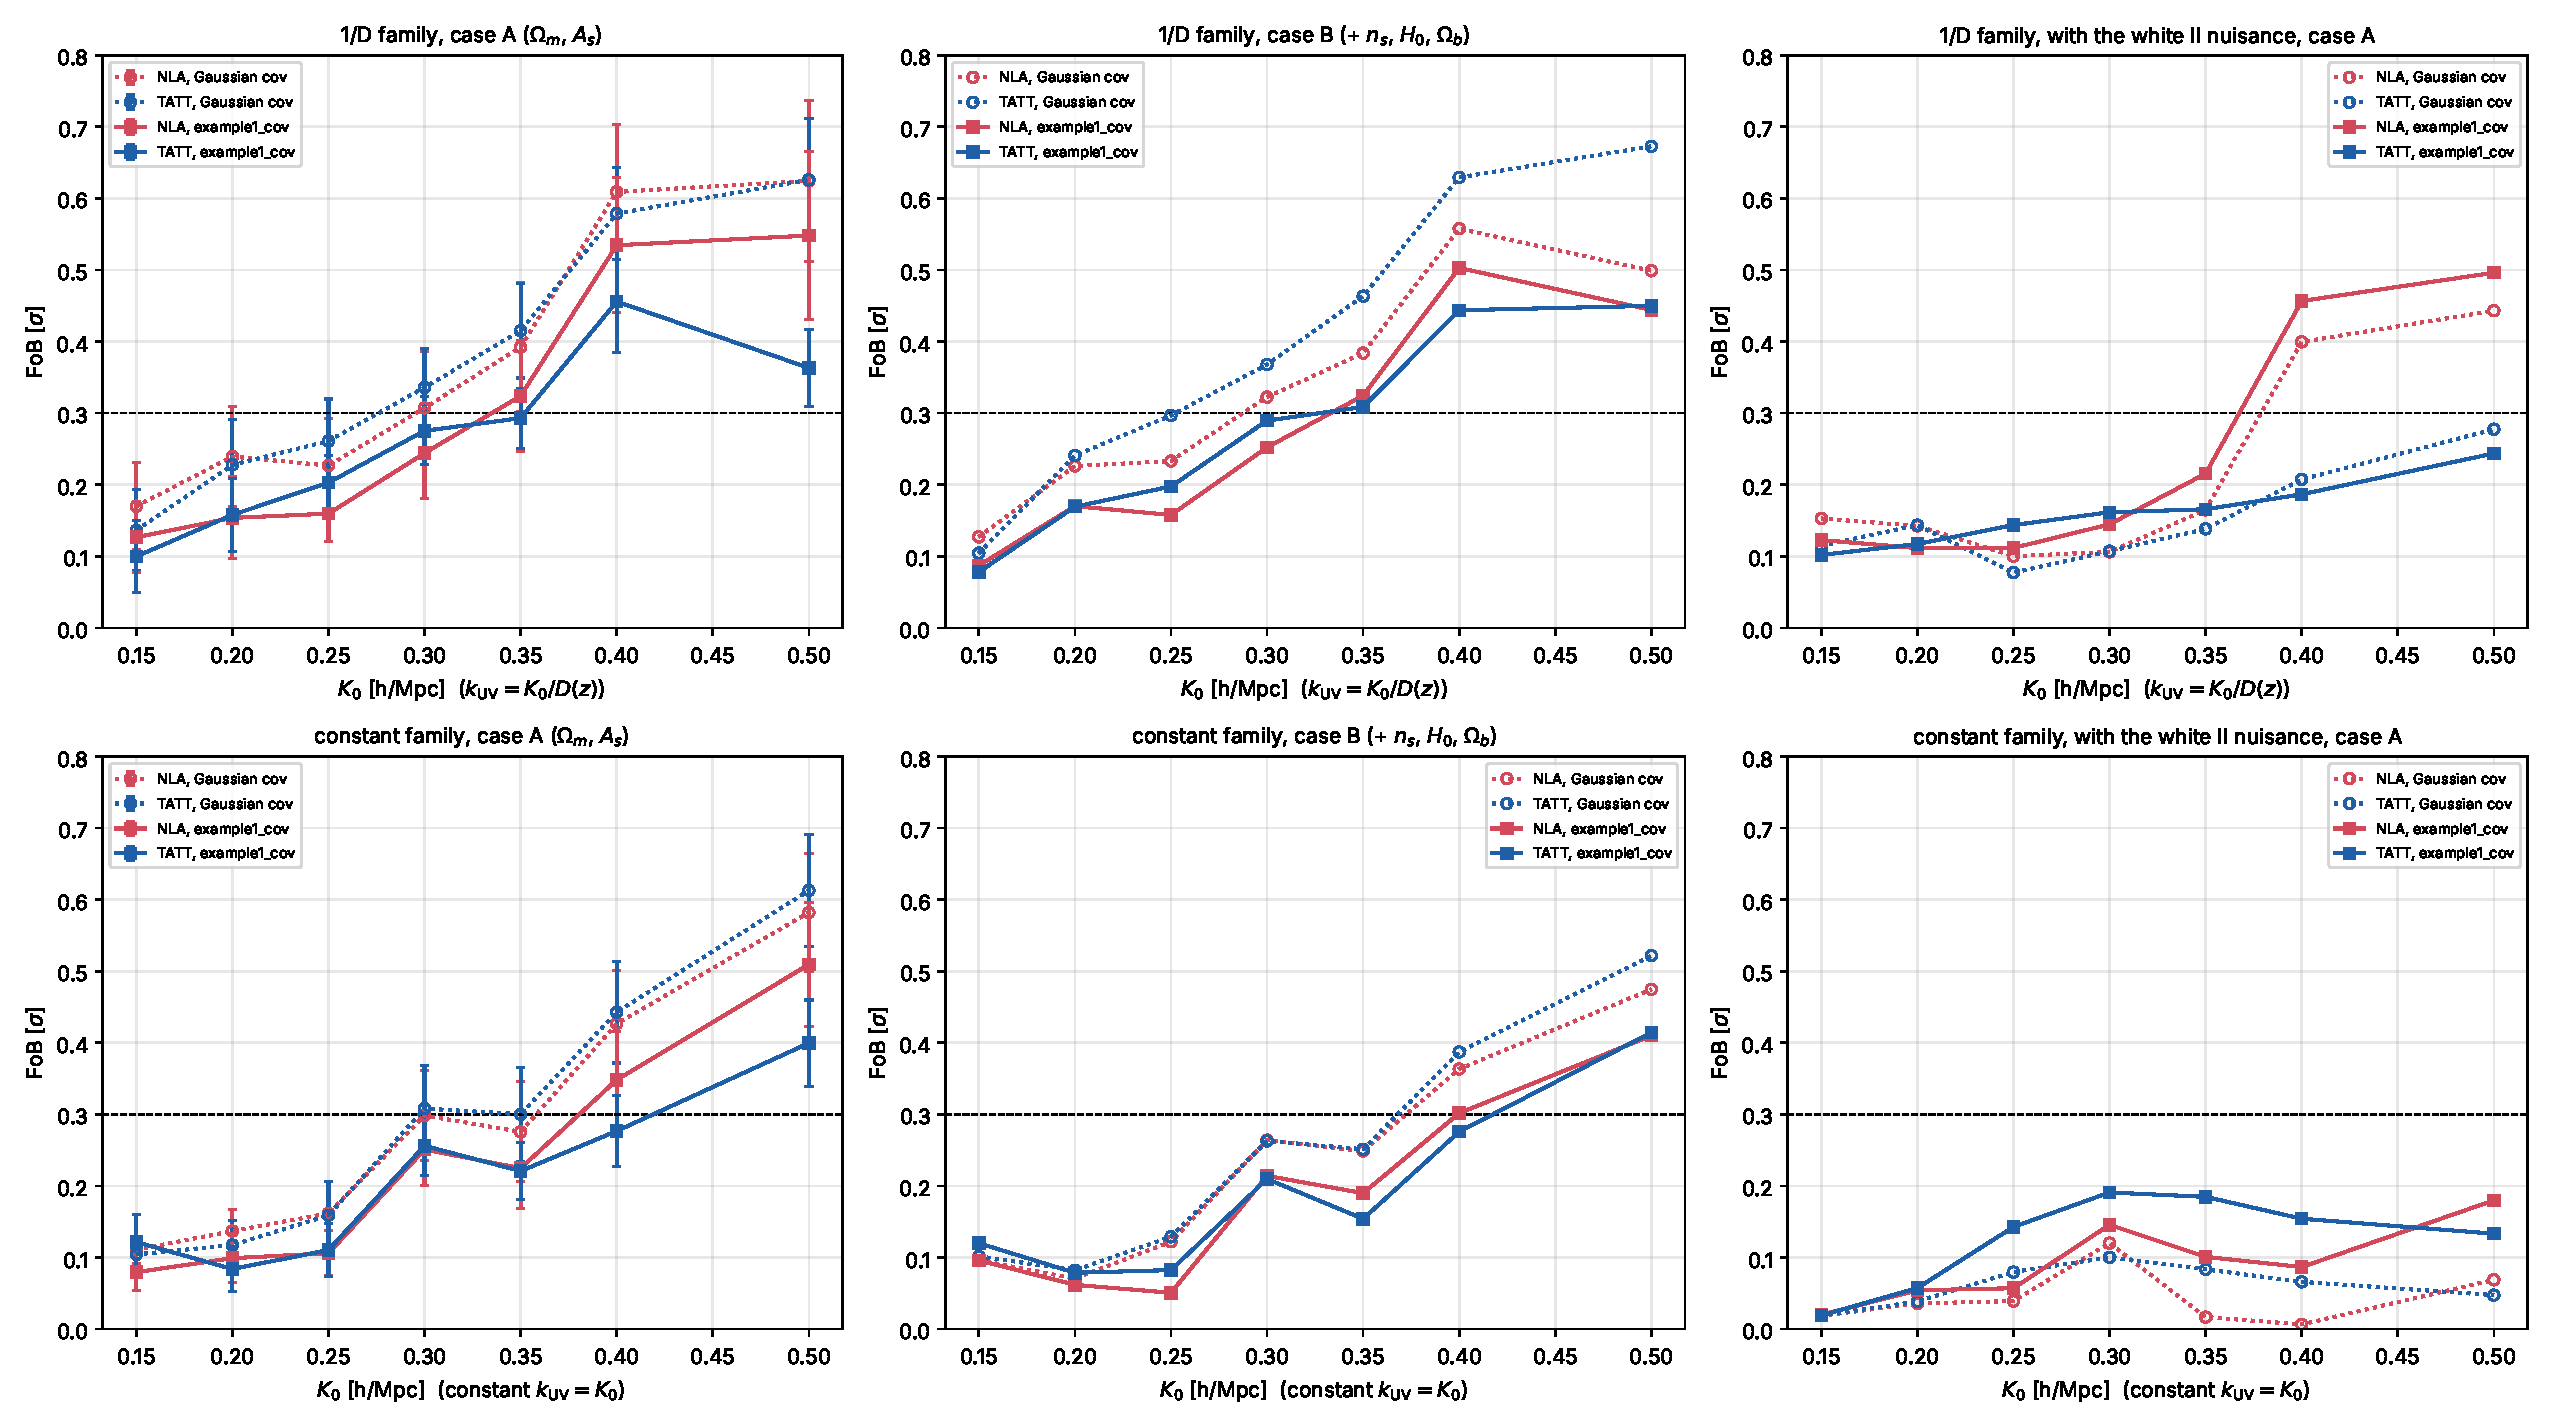
\includegraphics[width=\textwidth]{fig_ex1_fob}
\caption{Full-fit FoB against $K_0$ with the Gaussian covariance (open, dotted)
and \texttt{example1\_cov} (filled, solid): $1/D$ family (top), constant cut
(bottom); case A with FLAMINGO-noise error bars, case B, and with the white II
nuisance.}
\label{fig:ex1}
\end{figure}

\begin{table}[H]\centering\small
\caption{Full fits, Gaussian covariance versus \texttt{example1\_cov}.
$\sigma(S_8)$: case A, NLA (Fisher).}
\label{tab:ex1}
\resizebox{\textwidth}{!}{\begin{tabular}{llr cc cc cc c}\toprule
 & & & \multicolumn{2}{c}{FoB A (NLA / TATT)} & \multicolumn{2}{c}{FoB B (NLA / TATT)} & \multicolumn{2}{c}{+ white, A (NLA / TATT)} & $\sigma(S_8)$\\ \cmidrule(lr){4-5}\cmidrule(lr){6-7}\cmidrule(lr){8-9}
family & $K_0$ & pts & Gauss & example1 & Gauss & example1 & Gauss & example1 & Gauss $\to$ example1\\ \midrule
$1/D$ & 0.15 & 118 & 0.17 / 0.14 & 0.13 / 0.10 & 0.13 / 0.10 & 0.09 / 0.08 & 0.15 / 0.11 & 0.12 / 0.10 & 0.0112 $\to$ 0.0132\\
$1/D$ & 0.2 & 192 & 0.24 / 0.23 & 0.15 / 0.16 & 0.23 / 0.24 & 0.17 / 0.17 & 0.14 / 0.14 & 0.11 / 0.12 & 0.0073 $\to$ 0.0093\\
$1/D$ & 0.25 & 244 & 0.23 / 0.26 & 0.16 / 0.20 & 0.23 / 0.30 & 0.16 / 0.20 & 0.10 / 0.08 & 0.11 / 0.14 & 0.0060 $\to$ 0.0083\\
$1/D$ & 0.3 & 281 & 0.31 / 0.34 & 0.24 / 0.28 & 0.32 / 0.37 & 0.25 / 0.29 & 0.11 / 0.11 & 0.14 / 0.16 & 0.0048 $\to$ 0.0068\\
$1/D$ & 0.35 & 317 & 0.39 / 0.42 & 0.32 / 0.29 & 0.38 / 0.46 & 0.32 / 0.31 & 0.16 / 0.14 & 0.22 / 0.17 & 0.0045 $\to$ 0.0066\\
$1/D$ & 0.4 & 336 & 0.61 / 0.58 & 0.53 / 0.46 & 0.56 / 0.63 & 0.50 / 0.44 & 0.40 / 0.21 & 0.46 / 0.19 & 0.0040 $\to$ 0.0058\\
$1/D$ & 0.5 & 385 & 0.62 / 0.63 & 0.55 / 0.36 & 0.50 / 0.67 & 0.44 / 0.45 & 0.44 / 0.28 & 0.50 / 0.24 & 0.0035 $\to$ 0.0053\\
\midrule
constant & 0.15 & 94 & 0.11 / 0.10 & 0.08 / 0.12 & 0.10 / 0.10 & 0.10 / 0.12 & 0.02 / 0.02 & 0.02 / 0.02 & 0.0233 $\to$ 0.0274\\
constant & 0.2 & 151 & 0.14 / 0.12 & 0.10 / 0.08 & 0.07 / 0.08 & 0.06 / 0.08 & 0.04 / 0.04 & 0.05 / 0.06 & 0.0118 $\to$ 0.0152\\
constant & 0.25 & 197 & 0.16 / 0.16 & 0.11 / 0.11 & 0.12 / 0.13 & 0.05 / 0.08 & 0.04 / 0.08 & 0.06 / 0.14 & 0.0081 $\to$ 0.0108\\
constant & 0.3 & 239 & 0.30 / 0.31 & 0.25 / 0.26 & 0.26 / 0.26 & 0.21 / 0.21 & 0.12 / 0.10 & 0.15 / 0.19 & 0.0063 $\to$ 0.0085\\
constant & 0.35 & 266 & 0.28 / 0.30 & 0.22 / 0.22 & 0.25 / 0.25 & 0.19 / 0.15 & 0.02 / 0.08 & 0.10 / 0.18 & 0.0057 $\to$ 0.0081\\
constant & 0.4 & 292 & 0.43 / 0.44 & 0.35 / 0.28 & 0.36 / 0.39 & 0.30 / 0.28 & 0.01 / 0.07 & 0.09 / 0.15 & 0.0052 $\to$ 0.0075\\
constant & 0.5 & 335 & 0.58 / 0.61 & 0.51 / 0.40 & 0.47 / 0.52 & 0.41 / 0.41 & 0.07 / 0.05 & 0.18 / 0.13 & 0.0043 $\to$ 0.0063\\
\bottomrule\end{tabular}}
\end{table}

\begin{table}[H]\centering\small
\caption{Separate $\xi_\pm$ masks with \texttt{example1\_cov}, full fits.}
\label{tab:ex1split}
\begin{tabular}{lcc r cc c c}\toprule
model & $K_0^+$ & $K_0^-$ & pts & FoB A & FoB B & $\chi^2$ A & $\sigma(S_8)$ A\\ \midrule
NLA & 0.35 & 0.3 & 306 & 0.28 $\pm$ 0.08 & 0.27 & 1.94 & 0.0067\\
NLA & 0.4 & 0.3 & 315 & 0.38 $\pm$ 0.09 & 0.35 & 2.17 & 0.0061\\
TATT & 0.5 & 0.3 & 345 & 0.34 $\pm$ 0.08 & 0.28 & 2.64 & 0.0058\\
TATT & 0.4 & 0.3 & 315 & 0.27 $\pm$ 0.05 & 0.25 & 1.87 & 0.0066\\
\bottomrule\end{tabular}
\end{table}

\section{Recommendation and wording for the paper}\label{sec:rec}

\paragraph{Definition to adopt.} Strategy C as the defining criterion
(MAP shift with every parameter free, FoB $< 0.3$; FoB $+\,\sigma_{\rm noise}
< 0.3$ for the conservative variant), \emph{applied to each model separately},
the $1/D$ family as the mask shape, and A1, B1 and B2 as supporting evidence.
Nothing requires the two models to share a cut: the cut is a property of the
model, and showing that NLA needs a smaller $K_0$ (fewer points, larger
$\sigma(S_8)$) than TATT is a legitimate result. What the tests show is
\emph{when} that difference appears: it is hidden while the white II term
sits in the truth and no model has it, and it appears once that term is
modelled (Sec.~\ref{sec:D}, \ref{sec:ex1}). The paper should therefore make
the white-term decision explicit and present the model-specific cuts in the
configuration where it is modelled.

\begin{table}[H]\centering\small
\caption{Recommended cut sets with the production covariance
\texttt{example1\_cov} ($\alpha = 0.05$; GGL with $s > l$, $K_0^{\rm ggl} =
K_0^{\rm gc} = 0.2$ throughout). FoB case A (case B in brackets);
$\sigma(S_8)$ case A. Gaussian-covariance numbers in Sec.~\ref{sec:C} to
\ref{sec:D}.}
\label{tab:rec}
\resizebox{\textwidth}{!}{%
\begin{tabular}{llcccc}
\toprule
set & model & cosmic-shear cut & points & FoB & $\sigma(S_8)$\\
\midrule
model-specific, white nuisance (recommended) & NLA $+\,a_w$ & $K_0 = 0.35$ ($1/D$) & 317 & 0.22 & 0.0066\\
 & TATT $+\,a_w$ & $K_0 = 0.5$ ($1/D$) & 385 & 0.24 & 0.0055\\
\midrule
model-specific, constant cut, no white term & NLA & $k_{\rm UV} = 0.35$ & 266 & 0.22 (0.19) & 0.0081\\
 & TATT & $k_{\rm UV} = 0.4$ & 292 & 0.28 (0.28) & 0.0076\\
\midrule
model-specific, separate $\xi_\pm$ & NLA & $K_0^+ = 0.35$, $K_0^- = 0.3$ & 306 & 0.28 (0.27) & 0.0067\\
 & TATT & $K_0^+ = 0.4$, $K_0^- = 0.3$ & 315 & 0.27 (0.25) & 0.0066\\
\midrule
common $1/D$, no white term & both & $K_0 = 0.3$ & 281 & 0.24 / 0.28 (0.25 / 0.29) & 0.0068\\
conservative ($+\sigma_{\rm noise}$) & both & $K_0 = 0.25$ & 244 & 0.16 / 0.20 (0.16 / 0.20) & 0.0083\\
plan as written & both & $K_0 = 0.35$ & 317 & 0.32 / 0.29 (0.32 / 0.31) & 0.0066\\
\bottomrule
\end{tabular}}
\end{table}

\paragraph{A paragraph for the methods section.}
\begin{quote}\small
We define the cosmic-shear scale cuts with the IR/UV decomposition of
Saraivanov et al.\ (2026): an angular bin of $\xi_\pm^{ij}$ is kept if the
fraction of its signal from wavenumbers $k > \kuv(z) = K_0/D(z)$ is below
$\alpha = 0.05$. We fix $K_0$ separately for each IA model with an injection
test: the Roman data vector is computed with the GI and II spectra measured
in FLAMINGO, the analysis model (NLA or TATT, with power-law redshift
evolution) is fitted with all cosmological and nuisance parameters free, and
$K_0$ is the largest value for which the shift of the maximum-posterior
$(\Omega_m, S_8)$ stays below $0.3\sigma_{\rm 2D}$, after verifying that the
same test on a data vector generated with the analysis model returns zero.
The FLAMINGO spectra contain a white (one-halo) E-mode alignment term that
neither model includes and that contributes to $\xi_-$ on all angular scales;
we model it with one free amplitude in both analyses. NLA then requires $K_0
= 0.35\hmpc$, while TATT remains unbiased to $K_0 = 0.5\hmpc$, which keeps
21\% more data points and reduces $\sigma(S_8)$ by 17\%.
\end{quote}

\paragraph{Still to do before the cut is final.}
\begin{enumerate}[itemsep=1pt]
\item Done with \texttt{example1\_cov} (Sec.~\ref{sec:ex1}); repeat if the
  covariance is updated (the survey settings behind it are not documented).
\item Decide on the white term (truth or nuisance) and whether separate
  $\xi_\pm$ cuts are acceptable; together they decide between the rows of
  Table~\ref{tab:rec}.
\item Repeat the C test at the chosen mask with the chains (MAP and
  control-subtracted posterior mean).
\item If a second simulation or galaxy selection becomes available, use the
  spread between them for R2 (and as the envelope of D2).
\end{enumerate}

\begin{thebibliography}{9}\small
\bibitem{secco22} L.~F.~Secco, S.~Samuroff et al.\ (DES), \emph{Dark Energy
Survey Year 3 results: cosmology from cosmic shear and robustness to modeling
uncertainty}, PRD 105, 023515 (2022), arXiv:2105.13544; A.~Amon et al.,
arXiv:2105.13543.
\bibitem{krause21} E.~Krause et al.\ (DES), \emph{Dark Energy Survey Year 3
results: multi-probe modeling strategy and validation}, arXiv:2105.13548.
\bibitem{baldauf16} T.~Baldauf, M.~Mirbabayi, M.~Simonovi\'c, M.~Zaldarriaga,
\emph{LSS constraints with controlled theoretical uncertainties},
arXiv:1602.00674.
\bibitem{chudaykin21} A.~Chudaykin, M.~M.~Ivanov, M.~Simonovi\'c,
\emph{Optimizing large-scale structure data analysis with the theoretical
error likelihood}, PRD 103, 043525 (2021), arXiv:2009.10724.
\bibitem{saraivanov26} Saraivanov, Rubira, Miranda, Eifler (2026),
arXiv:2603.13031.
\end{thebibliography}

\appendix
\section{Code}
Base \texttt{/tmp/claude-0/out/roman\_dchi2/}; new code in \texttt{v4/}.
\begin{itemize}\sloppy
\item \texttt{v4/simfit.py}: per-snapshot NLA/TATT fitter with full
  parameter covariance (reproduces \texttt{v3/v3.npz} exactly).
\item \texttt{v4/sim\_strategies.py}: GoF and stability rules on the measured
  spectra, the volume scaling, noise and calibration realisations
  $\rightarrow$ \texttt{sim\_strategies.json}.
\item \texttt{v4/roman\_strategies.py}: Fisher precision of every mask,
  white-term linear response, tolerances (Eq.~\ref{eq:tol}), theory-error
  covariance fits (Eq.~\ref{eq:th}) $\rightarrow$
  \texttt{roman\_strategies.json}, \texttt{roman\_theory.json},
  \texttt{jacobians.npz}.
\item \texttt{v4/fisher\_white.py}: precision cost of the white nuisance
  $\rightarrow$ \texttt{fisher\_white.json}.
\item \texttt{v4/split\_pm.py}: linear-response scan of separate $\xi_+$ /
  $\xi_-$ cuts $\rightarrow$ \texttt{split\_pm.json};
  \texttt{v4/verify\_split.py}: full fits at selected separate masks
  $\rightarrow$ \texttt{verify\_split.json}.
\item Production covariance: \texttt{example1\_cov} downloaded from the LFS
  store (\texttt{media.githubusercontent.com}, SHA-256 checked), assembled to
  \texttt{cocoa/analysis/cov\_example1\_xi.npy} (and \texttt{\_3x2.npy});
  \texttt{v5/linear\_cov.py} (linear scan for any covariance $\rightarrow$
  \texttt{linear\_\{gauss,example1\}.json}); \texttt{v3/mask\_scan.py} with
  \texttt{COV}, \texttt{FAMS}, \texttt{OUTTAG} environment variables
  ($\rightarrow$ \texttt{mask\_scan\_ex1\_\{D1,flat\}.json});
  \texttt{v4/verify\_split.py} with \texttt{COV}, \texttt{CONF}
  ($\rightarrow$ \texttt{verify\_split\_ex1.json}); \texttt{v5/plot\_ex1.py}
  (\texttt{fig\_ex1\_fob}, \texttt{tab\_ex1.tex}, \texttt{tab\_ex1\_split.tex}).
\item \texttt{v4/plot\_strategies.py}: all figures, \texttt{derived.json};
  \texttt{v4/make\_tables.py}: the table bodies.
\item Earlier inputs: \texttt{v3/v3\_flamingo.py}, \texttt{v3/roman\_test.py},
  \texttt{v3/mask\_scan.py}, \texttt{v3/ggl3x2.py},
  \texttt{v3/knl\_scaling.py}, \texttt{v3/v3\_roman.py},
  \texttt{cocoa/translate\_matrix.py} (\texttt{J\_cells}),
  \texttt{v3s/run\_stitched.py}.
\end{itemize}
\end{document}
